\vspace*{-2.0cm}
\textbf{\Huge Results - Hard environment (1) }
\vspace{1.5cm}
\begin{tikzpicture}[remember picture,overlay]
   \node[anchor=south east,inner sep=20pt] at (current page.south east)
              {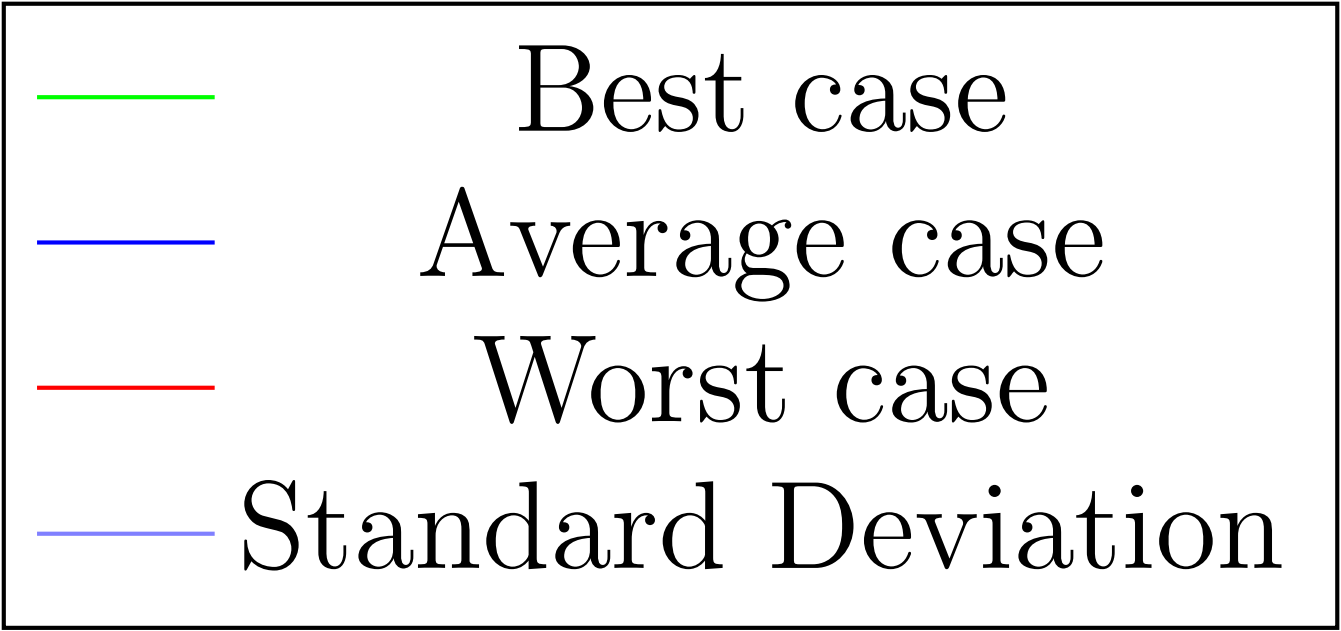
\includegraphics[scale=0.1]{chapters/res/generated_graph_legend.png}};
\end{tikzpicture}

\begin{figure}[H]
\vspace*{-1cm}
	\makebox[\linewidth][c]{%
	\begin{subfigure}[b]{0.7\textwidth}
		\centering
		\resizebox{0.9\linewidth}{!}{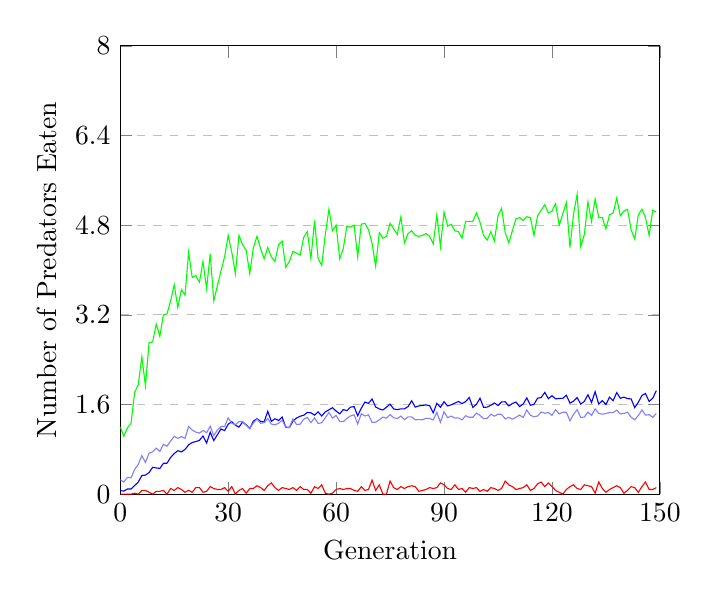
\begin{tikzpicture}
\begin{axis}[
	xlabel={Generation},
	ylabel={Number of Predators Eaten},
	xmin=0, xmax=150,
	ymin=0, ymax=8,
	xtick={0.0,30.0,60.0,90.0,120.0,150.0},
	ytick={0.0,1.6,3.2,4.800000000000001,6.4,8.0},
	ymajorgrids=true,
	grid style=dashed,
]

\addplot[
	color=green,
	]
	coordinates {
	(0,1.2)(1,1.0333333333333334)(2,1.1833333333333333)(3,1.2666666666666668)(4,1.8166666666666664)(5,1.95)(6,2.45)(7,1.9333333333333333)(8,2.7)(9,2.7166666666666663)(10,3.033333333333334)(11,2.8166666666666664)(12,3.1999999999999997)(13,3.2166666666666663)(14,3.45)(15,3.7333333333333334)(16,3.3333333333333335)(17,3.6500000000000004)(18,3.55)(19,4.316666666666666)(20,3.8666666666666663)(21,3.9000000000000004)(22,3.7833333333333337)(23,4.1499999999999995)(24,3.6666666666666665)(25,4.283333333333333)(26,3.45)(27,3.716666666666667)(28,3.9833333333333334)(29,4.2333333333333325)(30,4.616666666666666)(31,4.316666666666666)(32,3.9333333333333336)(33,4.616666666666667)(34,4.450000000000001)(35,4.35)(36,3.9333333333333336)(37,4.4)(38,4.6)(39,4.383333333333334)(40,4.2)(41,4.4)(42,4.2333333333333325)(43,4.1499999999999995)(44,4.449999999999999)(45,4.516666666666667)(46,4.05)(47,4.15)(48,4.333333333333335)(49,4.3)(50,4.2666666666666675)(51,4.583333333333334)(52,4.683333333333334)(53,4.2)(54,4.883333333333334)(55,4.200000000000001)(56,4.083333333333333)(57,4.633333333333333)(58,5.083333333333333)(59,4.699999999999999)(60,4.800000000000001)(61,4.2)(62,4.383333333333334)(63,4.783333333333332)(64,4.766666666666667)(65,4.799999999999999)(66,4.233333333333333)(67,4.8166666666666655)(68,4.833333333333333)(69,4.716666666666667)(70,4.466666666666667)(71,4.066666666666667)(72,4.666666666666666)(73,4.5666666666666655)(74,4.6)(75,4.833333333333333)(76,4.733333333333333)(77,4.633333333333333)(78,4.949999999999999)(79,4.483333333333333)(80,4.6499999999999995)(81,4.7)(82,4.616666666666667)(83,4.599999999999999)(84,4.616666666666666)(85,4.6499999999999995)(86,4.6)(87,4.466666666666668)(88,4.9833333333333325)(89,4.416666666666667)(90,5.033333333333333)(91,4.783333333333333)(92,4.8166666666666655)(93,4.699999999999998)(94,4.683333333333334)(95,4.566666666666666)(96,4.866666666666665)(97,4.866666666666667)(98,4.866666666666665)(99,5.016666666666666)(100,4.8500000000000005)(101,4.616666666666666)(102,4.533333333333332)(103,4.683333333333334)(104,4.516666666666667)(105,4.966666666666667)(106,5.1)(107,4.666666666666666)(108,4.483333333333333)(109,4.699999999999999)(110,4.916666666666668)(111,4.933333333333334)(112,4.883333333333334)(113,4.95)(114,4.9333333333333345)(115,4.616666666666666)(116,4.966666666666667)(117,5.066666666666666)(118,5.166666666666666)(119,5.016666666666667)(120,5.05)(121,5.183333333333334)(122,4.8)(123,4.999999999999999)(124,5.2)(125,4.4)(126,4.999999999999998)(127,5.35)(128,4.416666666666667)(129,4.633333333333333)(130,5.216666666666667)(131,4.866666666666667)(132,5.266666666666666)(133,4.933333333333334)(134,4.933333333333334)(135,4.733333333333333)(136,4.983333333333333)(137,5.016666666666667)(138,5.283333333333332)(139,4.966666666666666)(140,5.050000000000001)(141,5.083333333333332)(142,4.716666666666666)(143,4.550000000000001)(144,4.9833333333333325)(145,5.083333333333333)(146,4.933333333333333)(147,4.616666666666666)(148,5.066666666666666)(149,5.033333333333333)
	};
\addplot[
	color=blue,
	]
	coordinates {
	(0,0.0625)(1,0.05416666666666667)(2,0.09236111111111112)(3,0.09236111111111113)(4,0.15347222222222218)(5,0.2145833333333333)(6,0.33124999999999993)(7,0.34027777777777773)(8,0.38402777777777775)(9,0.47847222222222213)(10,0.467361111111111)(11,0.45833333333333326)(12,0.5499999999999998)(13,0.5520833333333334)(14,0.6541666666666668)(15,0.7249999999999999)(16,0.7743055555555558)(17,0.7548611111111111)(18,0.7972222222222223)(19,0.8805555555555554)(20,0.9208333333333333)(21,0.9375)(22,0.9590277777777778)(23,1.0375000000000003)(24,0.9124999999999999)(25,1.1055555555555554)(26,0.9555555555555554)(27,1.0604166666666666)(28,1.1638888888888888)(29,1.1326388888888888)(30,1.246527777777778)(31,1.29375)(32,1.2284722222222226)(33,1.195833333333333)(34,1.2875)(35,1.2368055555555557)(36,1.1701388888888893)(37,1.3020833333333333)(38,1.3465277777777778)(39,1.2979166666666668)(40,1.2881944444444446)(41,1.4784722222222226)(42,1.3006944444444444)(43,1.3451388888888889)(44,1.315277777777778)(45,1.3749999999999998)(46,1.1944444444444444)(47,1.1868055555555557)(48,1.3020833333333333)(49,1.3583333333333334)(50,1.3895833333333334)(51,1.407638888888889)(52,1.4576388888888887)(53,1.4513888888888888)(54,1.4097222222222223)(55,1.467361111111111)(56,1.3944444444444444)(57,1.4680555555555557)(58,1.5048611111111112)(59,1.542361111111111)(60,1.4819444444444443)(61,1.4326388888888892)(62,1.5083333333333333)(63,1.4902777777777783)(64,1.5527777777777776)(65,1.5618055555555557)(66,1.4)(67,1.5333333333333337)(68,1.6423611111111112)(69,1.6194444444444447)(70,1.697916666666667)(71,1.5541666666666667)(72,1.5208333333333335)(73,1.502083333333333)(74,1.551388888888889)(75,1.605555555555556)(76,1.5201388888888894)(77,1.507638888888889)(78,1.5222222222222224)(79,1.5222222222222224)(80,1.5624999999999998)(81,1.6666666666666663)(82,1.5520833333333333)(83,1.5743055555555556)(84,1.582638888888889)(85,1.5916666666666668)(86,1.5784722222222223)(87,1.4513888888888888)(88,1.619444444444445)(89,1.5499999999999996)(90,1.649305555555556)(91,1.5736111111111108)(92,1.5937500000000002)(93,1.623611111111111)(94,1.6541666666666666)(95,1.614583333333333)(96,1.6513888888888886)(97,1.7243055555555555)(98,1.5479166666666664)(99,1.6020833333333333)(100,1.7118055555555556)(101,1.5479166666666666)(102,1.5527777777777778)(103,1.5854166666666667)(104,1.6270833333333334)(105,1.5819444444444444)(106,1.6465277777777776)(107,1.6479166666666667)(108,1.5736111111111108)(109,1.6173611111111117)(110,1.6423611111111112)(111,1.5618055555555557)(112,1.607638888888889)(113,1.717361111111111)(114,1.5861111111111112)(115,1.6027777777777779)(116,1.7111111111111115)(117,1.724305555555555)(118,1.815277777777778)(119,1.7027777777777777)(120,1.7569444444444444)(121,1.7)(122,1.7069444444444444)(123,1.7090277777777778)(124,1.7652777777777775)(125,1.6243055555555554)(126,1.6597222222222223)(127,1.722222222222222)(128,1.60625)(129,1.6555555555555554)(130,1.7736111111111108)(131,1.6361111111111106)(132,1.8277777777777775)(133,1.6048611111111113)(134,1.6680555555555554)(135,1.5993055555555555)(136,1.73125)(137,1.6680555555555556)(138,1.8118055555555554)(139,1.7104166666666667)(140,1.7312500000000002)(141,1.7041666666666668)(142,1.6993055555555556)(143,1.543055555555555)(144,1.6402777777777777)(145,1.7597222222222222)(146,1.7958333333333334)(147,1.6541666666666666)(148,1.7097222222222224)(149,1.8465277777777775)
	};
\addplot[
	color=red,
	]
	coordinates {
	(0,0.0)(1,0.0)(2,0.0)(3,0.0)(4,0.016666666666666666)(5,0.0)(6,0.06666666666666667)(7,0.06666666666666667)(8,0.03333333333333333)(9,0.0)(10,0.05)(11,0.05)(12,0.06666666666666667)(13,0.0)(14,0.1)(15,0.06666666666666667)(16,0.11666666666666667)(17,0.08333333333333334)(18,0.03333333333333333)(19,0.06666666666666667)(20,0.03333333333333333)(21,0.11666666666666667)(22,0.11666666666666667)(23,0.03333333333333333)(24,0.05)(25,0.13333333333333333)(26,0.1)(27,0.08333333333333334)(28,0.08333333333333334)(29,0.11666666666666667)(30,0.05)(31,0.13333333333333333)(32,0.0)(33,0.06666666666666667)(34,0.1)(35,0.016666666666666666)(36,0.1)(37,0.1)(38,0.15)(39,0.11666666666666665)(40,0.06666666666666667)(41,0.15)(42,0.19999999999999998)(43,0.11666666666666667)(44,0.06666666666666667)(45,0.11666666666666667)(46,0.1)(47,0.08333333333333333)(48,0.11666666666666667)(49,0.06666666666666667)(50,0.13333333333333333)(51,0.08333333333333334)(52,0.08333333333333333)(53,0.016666666666666666)(54,0.13333333333333333)(55,0.1)(56,0.16666666666666666)(57,0.016666666666666666)(58,0.0)(59,0.016666666666666666)(60,0.08333333333333333)(61,0.1)(62,0.08333333333333333)(63,0.1)(64,0.1)(65,0.06666666666666667)(66,0.05)(67,0.13333333333333333)(68,0.06666666666666667)(69,0.08333333333333334)(70,0.24999999999999997)(71,0.06666666666666667)(72,0.16666666666666666)(73,0.0)(74,0.0)(75,0.2333333333333333)(76,0.11666666666666667)(77,0.08333333333333334)(78,0.13333333333333333)(79,0.09999999999999999)(80,0.13333333333333333)(81,0.15)(82,0.13333333333333333)(83,0.05)(84,0.06666666666666667)(85,0.08333333333333334)(86,0.11666666666666667)(87,0.1)(88,0.11666666666666667)(89,0.19999999999999998)(90,0.16666666666666666)(91,0.1)(92,0.08333333333333334)(93,0.16666666666666666)(94,0.08333333333333333)(95,0.1)(96,0.03333333333333333)(97,0.11666666666666667)(98,0.1)(99,0.11666666666666667)(100,0.05)(101,0.08333333333333334)(102,0.05)(103,0.11666666666666667)(104,0.09999999999999999)(105,0.06666666666666667)(106,0.1)(107,0.2333333333333333)(108,0.16666666666666666)(109,0.13333333333333333)(110,0.08333333333333333)(111,0.09999999999999999)(112,0.11666666666666667)(113,0.16666666666666666)(114,0.06666666666666667)(115,0.1)(116,0.18333333333333332)(117,0.21666666666666665)(118,0.13333333333333333)(119,0.19999999999999998)(120,0.13333333333333333)(121,0.06666666666666667)(122,0.03333333333333333)(123,0.0)(124,0.08333333333333333)(125,0.13333333333333333)(126,0.16666666666666666)(127,0.1)(128,0.08333333333333333)(129,0.16666666666666666)(130,0.15)(131,0.13333333333333333)(132,0.016666666666666666)(133,0.21666666666666665)(134,0.1)(135,0.03333333333333333)(136,0.08333333333333334)(137,0.11666666666666667)(138,0.15)(139,0.11666666666666667)(140,0.016666666666666666)(141,0.06666666666666667)(142,0.13333333333333333)(143,0.11666666666666667)(144,0.03333333333333333)(145,0.13333333333333333)(146,0.21666666666666665)(147,0.08333333333333334)(148,0.08333333333333333)(149,0.11666666666666667)
	};
\addplot[
	color=blue!50,
	]
	coordinates {
	(0,0.2567954586689933)(1,0.21629302775326373)(2,0.29920191485009023)(3,0.2917842860052699)(4,0.43938342611972053)(5,0.5298369903444883)(6,0.6873650424798703)(7,0.5659532033530428)(8,0.7297232936301211)(9,0.7562454027031459)(10,0.8224362592002558)(11,0.7604420089605098)(12,0.8884160818389348)(13,0.8558256675827959)(14,0.949200206948469)(15,1.0317455747521904)(16,0.9967686637648429)(17,1.0252715523862075)(18,0.9954271054797319)(19,1.206136175477242)(20,1.1415173509733176)(21,1.1079419833568562)(22,1.0880919702263587)(23,1.137001155109919)(24,1.0943035855783534)(25,1.2133976947676983)(26,1.045167325264568)(27,1.1444597482179737)(28,1.2057437200887111)(29,1.207006085856858)(30,1.3596970133505712)(31,1.2663909971018068)(32,1.2376025607000565)(33,1.2949883630135817)(34,1.2954343724501953)(35,1.2288708410924596)(36,1.1686294658132759)(37,1.2706605872502297)(38,1.3414481240707854)(39,1.264150269180343)(40,1.2742046493352315)(41,1.3490831072151277)(42,1.2500501865067586)(43,1.2375737939119473)(44,1.2633880233226185)(45,1.3202650000204446)(46,1.197479554826585)(47,1.1903955467406375)(48,1.3440609264808963)(49,1.2424043325695717)(50,1.2481356533589825)(51,1.3367010999474396)(52,1.3690356952150462)(53,1.275743932705493)(54,1.3614850755144656)(55,1.2600310621842614)(56,1.2745093554985076)(57,1.361182498474822)(58,1.4569455141031105)(59,1.356445306887592)(60,1.4046999807623346)(61,1.2959300380622536)(62,1.293074279873345)(63,1.354286951624945)(64,1.3952056236588637)(65,1.4150506451628497)(66,1.2529736101027726)(67,1.4357940836252543)(68,1.3944339029414623)(69,1.4159059009838726)(70,1.2789197138192603)(71,1.2840493739316572)(72,1.3261680493358272)(73,1.3753443259570692)(74,1.3550459424269616)(75,1.4187104766158183)(76,1.363266470358261)(77,1.3483264132399708)(78,1.3934828964094277)(79,1.329994211296116)(80,1.378364512826987)(81,1.377828735532433)(82,1.3260238723402658)(83,1.3304993318180296)(84,1.3267253015240073)(85,1.3535989021598125)(86,1.35025706436527)(87,1.3235071445105966)(88,1.4604813466608608)(89,1.28127439821142)(90,1.470162284717902)(91,1.364341394001647)(92,1.392461287390359)(93,1.3565811952094564)(94,1.3614993997368516)(95,1.3241004828149456)(96,1.3996515364229842)(97,1.3710041273057996)(98,1.371718036039779)(99,1.4468404464847928)(100,1.4046186835167647)(101,1.346464299416398)(102,1.3531902904051816)(103,1.4272891255473228)(104,1.3915631833793658)(105,1.4265844183796499)(106,1.4226527573203374)(107,1.342168301343959)(108,1.3701282904084517)(109,1.3384810713146797)(110,1.3720313722187614)(111,1.4111536257843982)(112,1.3668462715075946)(113,1.5007794996073955)(114,1.4070458745893863)(115,1.3808119367266334)(116,1.394442224909498)(117,1.4650073572029583)(118,1.443160942058554)(119,1.4565992214116765)(120,1.4055073672201828)(121,1.5082402418775767)(122,1.4319743496640134)(123,1.4613611003038145)(124,1.4601469545553467)(125,1.3076995324109888)(126,1.4237984753090769)(127,1.5078658177238164)(128,1.368939341391302)(129,1.3758217751105597)(130,1.4647220952274642)(131,1.4038274578024166)(132,1.5235658440892983)(133,1.4399870181163297)(134,1.4272968610701615)(135,1.4374197605233643)(136,1.4581450173104689)(137,1.4543316025882906)(138,1.499030213581117)(139,1.4313398215750164)(140,1.4394016109833991)(141,1.4619107340953532)(142,1.3740528031658596)(143,1.3255783287870362)(144,1.402239531501261)(145,1.503277663037369)(146,1.4095204305005509)(147,1.4190285375644207)(148,1.3704329774235906)(149,1.43738691981063)
	};
\end{axis}
\end{tikzpicture}
}
		\caption{Some sample caption}
	\end{subfigure}%
	\begin{subfigure}[b]{0.7\textwidth}	
		\centering
		\resizebox{0.9\linewidth}{!}{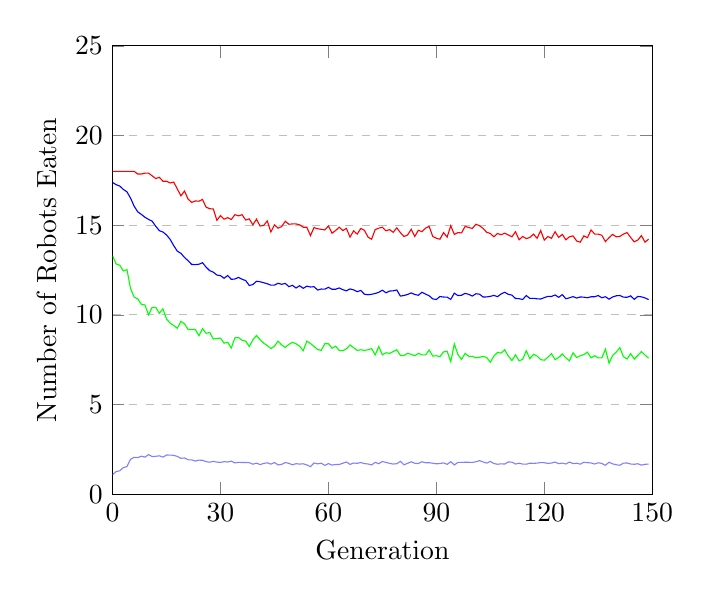
\begin{tikzpicture}
\begin{axis}[
	xlabel={Generation},
	ylabel={Number of Robots Eaten},
	xmin=0, xmax=150,
	ymin=0, ymax=25,
	xtick={0.0,30.0,60.0,90.0,120.0,150.0},
	ytick={0.0,5.0,10.0,15.0,20.0,25.0},
	ymajorgrids=true,
	grid style=dashed,
]

\addplot[
	color=red,
	]
	coordinates {
	(0,18.0)(1,18.0)(2,18.0)(3,18.0)(4,18.0)(5,18.0)(6,18.0)(7,17.85)(8,17.85)(9,17.9)(10,17.9)(11,17.750000000000004)(12,17.6)(13,17.666666666666668)(14,17.45)(15,17.45)(16,17.35)(17,17.4)(18,17.01666666666667)(19,16.633333333333336)(20,16.900000000000002)(21,16.450000000000003)(22,16.26666666666667)(23,16.35)(24,16.333333333333332)(25,16.433333333333337)(26,16.000000000000004)(27,15.91666666666667)(28,15.9)(29,15.266666666666666)(30,15.533333333333333)(31,15.333333333333332)(32,15.416666666666666)(33,15.316666666666666)(34,15.583333333333332)(35,15.516666666666667)(36,15.583333333333334)(37,15.283333333333335)(38,15.349999999999998)(39,15.016666666666666)(40,15.333333333333336)(41,14.949999999999998)(42,14.983333333333333)(43,15.233333333333334)(44,14.616666666666665)(45,15.016666666666666)(46,14.833333333333336)(47,14.916666666666666)(48,15.216666666666667)(49,15.049999999999999)(50,15.066666666666668)(51,15.066666666666665)(52,15.016666666666667)(53,14.883333333333333)(54,14.883333333333335)(55,14.416666666666666)(56,14.866666666666667)(57,14.8)(58,14.766666666666666)(59,14.733333333333334)(60,14.950000000000001)(61,14.549999999999997)(62,14.700000000000003)(63,14.883333333333335)(64,14.7)(65,14.81666666666667)(66,14.333333333333334)(67,14.683333333333335)(68,14.500000000000002)(69,14.816666666666666)(70,14.716666666666667)(71,14.33333333333333)(72,14.216666666666667)(73,14.749999999999998)(74,14.833333333333336)(75,14.883333333333336)(76,14.683333333333334)(77,14.750000000000004)(78,14.6)(79,14.85)(80,14.583333333333336)(81,14.366666666666665)(82,14.45)(83,14.766666666666666)(84,14.366666666666665)(85,14.716666666666665)(86,14.633333333333335)(87,14.833333333333332)(88,14.933333333333335)(89,14.366666666666667)(90,14.266666666666664)(91,14.216666666666667)(92,14.583333333333336)(93,14.333333333333332)(94,14.966666666666669)(95,14.48333333333333)(96,14.583333333333334)(97,14.566666666666666)(98,14.933333333333334)(99,14.866666666666665)(100,14.816666666666666)(101,15.05)(102,14.966666666666667)(103,14.816666666666666)(104,14.600000000000001)(105,14.533333333333333)(106,14.350000000000001)(107,14.533333333333333)(108,14.466666666666665)(109,14.55)(110,14.450000000000003)(111,14.35)(112,14.633333333333333)(113,14.183333333333335)(114,14.366666666666665)(115,14.249999999999998)(116,14.316666666666666)(117,14.499999999999996)(118,14.266666666666666)(119,14.700000000000001)(120,14.166666666666664)(121,14.366666666666667)(122,14.266666666666667)(123,14.633333333333333)(124,14.316666666666668)(125,14.483333333333333)(126,14.183333333333335)(127,14.349999999999998)(128,14.4)(129,14.116666666666669)(130,14.049999999999995)(131,14.400000000000004)(132,14.3)(133,14.733333333333336)(134,14.5)(135,14.5)(136,14.433333333333335)(137,14.083333333333334)(138,14.3)(139,14.48333333333333)(140,14.350000000000001)(141,14.366666666666665)(142,14.5)(143,14.583333333333332)(144,14.316666666666668)(145,14.066666666666663)(146,14.166666666666664)(147,14.416666666666668)(148,14.049999999999997)(149,14.216666666666667)
	};
\addplot[
	color=blue,
	]
	coordinates {
	(0,17.38125)(1,17.25486111111111)(2,17.179166666666664)(3,16.991666666666667)(4,16.856944444444444)(5,16.506944444444443)(6,16.056250000000002)(7,15.74027777777778)(8,15.6)(9,15.439583333333335)(10,15.318749999999998)(11,15.221527777777782)(12,14.937500000000002)(13,14.691666666666666)(14,14.615972222222222)(15,14.452083333333334)(16,14.206944444444442)(17,13.854861111111113)(18,13.549999999999999)(19,13.428472222222224)(20,13.195833333333331)(21,13.01527777777778)(22,12.805555555555554)(23,12.800000000000002)(24,12.81875)(25,12.905555555555555)(26,12.656944444444445)(27,12.461111111111112)(28,12.378472222222223)(29,12.216666666666669)(30,12.183333333333337)(31,12.037499999999998)(32,12.190972222222223)(33,11.977777777777778)(34,11.996527777777779)(35,12.08611111111111)(36,11.981249999999998)(37,11.910416666666666)(38,11.634027777777774)(39,11.686805555555553)(40,11.868750000000002)(41,11.844444444444445)(42,11.790277777777776)(43,11.731944444444443)(44,11.652777777777779)(45,11.654166666666669)(46,11.760416666666668)(47,11.699305555555554)(48,11.751388888888888)(49,11.570833333333335)(50,11.643055555555556)(51,11.495833333333332)(52,11.62013888888889)(53,11.477083333333335)(54,11.597222222222221)(55,11.549305555555554)(56,11.569444444444443)(57,11.38125)(58,11.436805555555555)(59,11.431944444444447)(60,11.533333333333337)(61,11.42222222222222)(62,11.426388888888889)(63,11.496527777777777)(64,11.401388888888889)(65,11.3375)(66,11.443750000000001)(67,11.388194444444444)(68,11.288194444444443)(69,11.357638888888886)(70,11.14861111111111)(71,11.118055555555555)(72,11.145138888888889)(73,11.188194444444447)(74,11.256944444444445)(75,11.372916666666667)(76,11.227083333333333)(77,11.32291666666667)(78,11.3375)(79,11.384722222222221)(80,11.042361111111111)(81,11.07777777777778)(82,11.135416666666668)(83,11.218055555555557)(84,11.135416666666668)(85,11.088194444444444)(86,11.258333333333331)(87,11.153472222222224)(88,11.061805555555559)(89,10.885416666666664)(90,10.85486111111111)(91,11.019444444444447)(92,10.990972222222222)(93,10.983333333333334)(94,10.859722222222222)(95,11.207638888888887)(96,11.072916666666668)(97,11.090277777777775)(98,11.195833333333331)(99,11.139583333333334)(100,11.044444444444446)(101,11.174305555555557)(102,11.149305555555557)(103,10.990277777777779)(104,10.997222222222222)(105,11.02986111111111)(106,11.082638888888889)(107,11.012500000000001)(108,11.163194444444445)(109,11.255555555555556)(110,11.141666666666666)(111,11.09861111111111)(112,10.91111111111111)(113,10.897222222222219)(114,10.853472222222223)(115,11.075694444444446)(116,10.9125)(117,10.919444444444444)(118,10.891666666666667)(119,10.879861111111111)(120,10.956944444444444)(121,11.025000000000002)(122,11.022222222222222)(123,11.106250000000001)(124,10.975000000000001)(125,11.125694444444443)(126,10.89236111111111)(127,10.94861111111111)(128,11.015277777777778)(129,10.935416666666669)(130,10.995138888888889)(131,10.982638888888888)(132,10.951388888888888)(133,11.004166666666668)(134,11.00486111111111)(135,11.072916666666666)(136,10.95)(137,11.008333333333335)(138,10.872916666666667)(139,10.99236111111111)(140,11.059722222222225)(141,11.077083333333334)(142,10.986111111111107)(143,10.975)(144,11.056249999999999)(145,10.858333333333333)(146,11.026388888888887)(147,11.002083333333333)(148,10.941666666666663)(149,10.849999999999998)
	};
\addplot[
	color=green,
	]
	coordinates {
	(0,13.299999999999999)(1,12.833333333333334)(2,12.766666666666667)(3,12.450000000000001)(4,12.516666666666667)(5,11.466666666666665)(6,10.983333333333333)(7,10.883333333333335)(8,10.583333333333334)(9,10.55)(10,10.0)(11,10.416666666666668)(12,10.416666666666666)(13,10.083333333333334)(14,10.333333333333332)(15,9.766666666666666)(16,9.533333333333335)(17,9.4)(18,9.249999999999998)(19,9.633333333333335)(20,9.500000000000002)(21,9.183333333333332)(22,9.183333333333335)(23,9.183333333333334)(24,8.833333333333332)(25,9.233333333333334)(26,8.966666666666667)(27,9.016666666666667)(28,8.650000000000002)(29,8.683333333333334)(30,8.7)(31,8.416666666666668)(32,8.466666666666669)(33,8.15)(34,8.716666666666669)(35,8.733333333333333)(36,8.583333333333334)(37,8.533333333333333)(38,8.233333333333334)(39,8.600000000000001)(40,8.85)(41,8.616666666666667)(42,8.416666666666666)(43,8.283333333333335)(44,8.116666666666667)(45,8.250000000000002)(46,8.533333333333335)(47,8.316666666666666)(48,8.183333333333334)(49,8.350000000000001)(50,8.466666666666667)(51,8.383333333333333)(52,8.250000000000002)(53,8.0)(54,8.533333333333333)(55,8.400000000000002)(56,8.233333333333334)(57,8.066666666666666)(58,8.016666666666667)(59,8.383333333333335)(60,8.383333333333335)(61,8.133333333333333)(62,8.250000000000002)(63,8.016666666666666)(64,7.999999999999999)(65,8.1)(66,8.316666666666666)(67,8.166666666666668)(68,8.016666666666667)(69,8.05)(70,8.016666666666667)(71,8.05)(72,8.116666666666667)(73,7.766666666666668)(74,8.233333333333334)(75,7.766666666666666)(76,7.8833333333333355)(77,7.850000000000002)(78,7.95)(79,8.05)(80,7.733333333333335)(81,7.733333333333333)(82,7.850000000000002)(83,7.799999999999998)(84,7.716666666666669)(85,7.850000000000001)(86,7.7666666666666675)(87,7.766666666666667)(88,8.033333333333333)(89,7.699999999999999)(90,7.716666666666667)(91,7.666666666666668)(92,7.933333333333333)(93,7.966666666666669)(94,7.3833333333333355)(95,8.383333333333333)(96,7.783333333333332)(97,7.516666666666667)(98,7.8500000000000005)(99,7.683333333333332)(100,7.683333333333334)(101,7.6)(102,7.633333333333335)(103,7.683333333333335)(104,7.616666666666667)(105,7.3500000000000005)(106,7.699999999999999)(107,7.900000000000001)(108,7.866666666666667)(109,8.05)(110,7.700000000000002)(111,7.449999999999998)(112,7.7666666666666675)(113,7.433333333333334)(114,7.5166666666666675)(115,8.000000000000002)(116,7.550000000000001)(117,7.800000000000002)(118,7.699999999999998)(119,7.500000000000001)(120,7.466666666666667)(121,7.633333333333334)(122,7.833333333333335)(123,7.5)(124,7.616666666666667)(125,7.816666666666668)(126,7.600000000000001)(127,7.433333333333335)(128,7.883333333333335)(129,7.616666666666669)(130,7.716666666666667)(131,7.783333333333333)(132,7.916666666666668)(133,7.600000000000001)(134,7.716666666666668)(135,7.6000000000000005)(136,7.6)(137,8.083333333333336)(138,7.3)(139,7.733333333333334)(140,7.916666666666666)(141,8.166666666666668)(142,7.666666666666665)(143,7.533333333333331)(144,7.833333333333335)(145,7.533333333333334)(146,7.733333333333333)(147,7.949999999999999)(148,7.75)(149,7.583333333333333)
	};
\addplot[
	color=blue!50,
	]
	coordinates {
	(0,1.0845553930560614)(1,1.2569338975860094)(2,1.3017983326147198)(3,1.4808281183298073)(4,1.5368804893331904)(5,1.9414565911936879)(6,2.052438579185581)(7,2.0371261762853474)(8,2.1147316306649677)(9,2.0644475504300304)(10,2.2027891777900086)(11,2.0974227426931784)(12,2.1099997400216015)(13,2.1365971943227424)(14,2.0647111376362184)(15,2.179269219016812)(16,2.1789261262717727)(17,2.162328782803921)(18,2.103319594799526)(19,1.9964660276363264)(20,2.0169980862615615)(21,1.913533661859874)(22,1.9103853828804676)(23,1.845100614466328)(24,1.894540488688379)(25,1.8879539015113127)(26,1.810227541690253)(27,1.7796893021754037)(28,1.8263200645558042)(29,1.7852800826213544)(30,1.7691009754808276)(31,1.811943203641366)(32,1.7894988814919188)(33,1.8413266258642207)(34,1.7394693229722307)(35,1.773349402933656)(36,1.7626908875390925)(37,1.7650052221532893)(38,1.755056004005871)(39,1.6694770087006683)(40,1.7288978782220779)(41,1.6490058014997229)(42,1.7108563175169367)(43,1.7469725300722967)(44,1.672308898221016)(45,1.76198673162835)(46,1.6269161630694104)(47,1.6604690006506309)(48,1.7601992732088814)(49,1.7157687549258058)(50,1.6355864658257606)(51,1.698269369571266)(52,1.6745451327979028)(53,1.6925176675911218)(54,1.6281014739767259)(55,1.5343649292329151)(56,1.73725373034437)(57,1.687577789854123)(58,1.7239662513624021)(59,1.6012136998670252)(60,1.7033664792675265)(61,1.6190976867359137)(62,1.6522349123607005)(63,1.653489949972742)(64,1.7204828953420213)(65,1.7947295405532513)(66,1.657043752441505)(67,1.734310023298112)(68,1.7185881263641383)(69,1.7624345107154464)(70,1.7026454936666648)(71,1.680907611237149)(72,1.6283055633317973)(73,1.7731331248221651)(74,1.6961798680916977)(75,1.8194971275218461)(76,1.7705839796084886)(77,1.7149739141094633)(78,1.6787291489883853)(79,1.6967526155660022)(80,1.8263891833335264)(81,1.6360192742802997)(82,1.7170426061537163)(83,1.8036798139515082)(84,1.7196475813775935)(85,1.7054149328387864)(86,1.8057918093378942)(87,1.7498508057083495)(88,1.7513803095709037)(89,1.7244946059843673)(90,1.6910670844633653)(91,1.7061525198522098)(92,1.743773515582125)(93,1.6601675697537441)(94,1.8085626729988915)(95,1.6268270636065576)(96,1.768183265427153)(97,1.7680085311295117)(98,1.7789371524196773)(99,1.7749789380496006)(100,1.7686108900810018)(101,1.805258918689446)(102,1.8662796521010188)(103,1.7930151082124868)(104,1.7283498944904854)(105,1.8222028549189824)(106,1.7064253771117204)(107,1.6664239861862777)(108,1.6902588219290244)(109,1.6754660062012563)(110,1.793923798977226)(111,1.7851497722087277)(112,1.6784761343327914)(113,1.724181263660402)(114,1.6753377493600876)(115,1.6688694545073928)(116,1.7249232675298631)(117,1.7170341456605627)(118,1.729609585662609)(119,1.7598630286745318)(120,1.752173949633828)(121,1.7130797373799131)(122,1.734320922850237)(123,1.7894755728712155)(124,1.6974486819961991)(125,1.7308083656229294)(126,1.6814474617269677)(127,1.7876011258282214)(128,1.702369609831248)(129,1.7243512522623894)(130,1.67156201349268)(131,1.7759576866332487)(132,1.7543351440765447)(133,1.7394384821476907)(134,1.6784968639697497)(135,1.7468641555926465)(136,1.711345018847415)(137,1.6089217547982122)(138,1.7777003360526693)(139,1.687782262115383)(140,1.6389884908846712)(141,1.6105802017887851)(142,1.72834116299074)(143,1.7380203270924734)(144,1.6792547265312)(145,1.6648842371869519)(146,1.6942252906511823)(147,1.6172386476929739)(148,1.6625562179078772)(149,1.675906672645179)
	};
\end{axis}
\end{tikzpicture}
}
		\caption{Some sample caption}
		\label{fig:hard-robots-eaten}
	\end{subfigure}%
}
\\
\\
\\
	\makebox[\linewidth][c]{%
	\begin{subfigure}[b]{0.7\textwidth}
		\centering
		\resizebox{0.9\linewidth}{!}{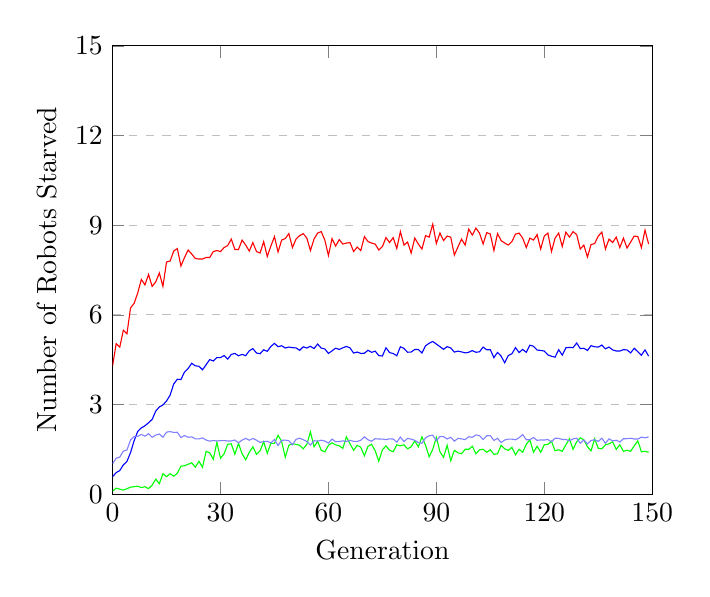
\begin{tikzpicture}
\begin{axis}[
	xlabel={Generation},
	ylabel={Number of Robots Starved},
	xmin=0, xmax=150,
	ymin=0, ymax=15,
	xtick={0.0,30.0,60.0,90.0,120.0,150.0},
	ytick={0.0,3.0,6.0,9.0,12.0,15.0},
	ymajorgrids=true,
	grid style=dashed,
]

\addplot[
	color=red,
	]
	coordinates {
	(0,4.283333333333333)(1,5.033333333333333)(2,4.916666666666666)(3,5.483333333333333)(4,5.366666666666665)(5,6.233333333333333)(6,6.383333333333333)(7,6.7333333333333325)(8,7.183333333333333)(9,7.0)(10,7.35)(11,6.949999999999999)(12,7.1)(13,7.400000000000001)(14,6.95)(15,7.766666666666667)(16,7.800000000000001)(17,8.133333333333333)(18,8.216666666666667)(19,7.633333333333334)(20,7.916666666666669)(21,8.166666666666668)(22,8.033333333333335)(23,7.883333333333335)(24,7.866666666666667)(25,7.866666666666667)(26,7.916666666666667)(27,7.916666666666667)(28,8.116666666666667)(29,8.15)(30,8.116666666666667)(31,8.25)(32,8.316666666666668)(33,8.533333333333333)(34,8.183333333333335)(35,8.183333333333334)(36,8.500000000000002)(37,8.333333333333334)(38,8.133333333333335)(39,8.416666666666668)(40,8.116666666666667)(41,8.066666666666666)(42,8.45)(43,7.95)(44,8.3)(45,8.616666666666667)(46,8.1)(47,8.500000000000002)(48,8.55)(49,8.716666666666667)(50,8.25)(51,8.533333333333335)(52,8.650000000000002)(53,8.716666666666667)(54,8.566666666666666)(55,8.15)(56,8.533333333333333)(57,8.733333333333334)(58,8.783333333333333)(59,8.500000000000004)(60,7.983333333333333)(61,8.55)(62,8.3)(63,8.516666666666667)(64,8.366666666666667)(65,8.400000000000002)(66,8.416666666666666)(67,8.116666666666667)(68,8.266666666666667)(69,8.150000000000002)(70,8.616666666666667)(71,8.450000000000001)(72,8.399999999999999)(73,8.366666666666669)(74,8.166666666666668)(75,8.283333333333333)(76,8.583333333333334)(77,8.416666666666668)(78,8.583333333333334)(79,8.216666666666665)(80,8.783333333333335)(81,8.333333333333332)(82,8.433333333333334)(83,8.066666666666666)(84,8.566666666666666)(85,8.366666666666665)(86,8.2)(87,8.65)(88,8.6)(89,9.033333333333333)(90,8.383333333333333)(91,8.733333333333333)(92,8.483333333333333)(93,8.633333333333333)(94,8.600000000000001)(95,8.000000000000002)(96,8.266666666666666)(97,8.533333333333331)(98,8.333333333333334)(99,8.866666666666665)(100,8.666666666666666)(101,8.900000000000002)(102,8.733333333333334)(103,8.366666666666667)(104,8.750000000000002)(105,8.700000000000001)(106,8.150000000000002)(107,8.716666666666667)(108,8.483333333333334)(109,8.399999999999999)(110,8.333333333333332)(111,8.450000000000001)(112,8.700000000000001)(113,8.733333333333333)(114,8.56666666666667)(115,8.25)(116,8.566666666666668)(117,8.500000000000002)(118,8.683333333333335)(119,8.2)(120,8.633333333333333)(121,8.733333333333334)(122,8.116666666666667)(123,8.566666666666668)(124,8.733333333333334)(125,8.283333333333333)(126,8.766666666666667)(127,8.6)(128,8.783333333333333)(129,8.683333333333332)(130,8.2)(131,8.333333333333332)(132,7.933333333333335)(133,8.35)(134,8.383333333333335)(135,8.633333333333333)(136,8.76666666666667)(137,8.2)(138,8.533333333333335)(139,8.416666666666668)(140,8.599999999999998)(141,8.249999999999998)(142,8.566666666666668)(143,8.23333333333333)(144,8.433333333333334)(145,8.633333333333335)(146,8.616666666666667)(147,8.249999999999998)(148,8.833333333333334)(149,8.366666666666667)
	};
\addplot[
	color=blue,
	]
	coordinates {
	(0,0.5847222222222224)(1,0.7194444444444447)(2,0.7881944444444445)(3,0.9784722222222224)(4,1.09375)(5,1.392361111111111)(6,1.789583333333333)(7,2.0993055555555555)(8,2.2166666666666663)(9,2.2868055555555555)(10,2.3881944444444443)(11,2.4993055555555554)(12,2.778472222222222)(13,2.916666666666667)(14,2.983333333333334)(15,3.116666666666666)(16,3.3118055555555563)(17,3.6868055555555554)(18,3.843055555555557)(19,3.8333333333333335)(20,4.085416666666665)(21,4.202083333333333)(22,4.379166666666667)(23,4.290972222222222)(24,4.279861111111113)(25,4.1618055555555555)(26,4.328472222222223)(27,4.502083333333332)(28,4.456250000000001)(29,4.569444444444444)(30,4.568055555555556)(31,4.636111111111111)(32,4.516666666666667)(33,4.674305555555556)(34,4.706944444444443)(35,4.628472222222223)(36,4.675694444444445)(37,4.631944444444445)(38,4.795138888888889)(39,4.8687499999999995)(40,4.7222222222222205)(41,4.697222222222222)(42,4.828472222222222)(43,4.779166666666666)(44,4.940277777777777)(45,5.045138888888889)(46,4.9319444444444445)(47,4.965277777777778)(48,4.888888888888888)(49,4.9208333333333325)(50,4.9006944444444445)(51,4.8909722222222225)(52,4.811111111111111)(53,4.929166666666665)(54,4.890277777777778)(55,4.94513888888889)(56,4.872222222222222)(57,5.020833333333332)(58,4.886805555555555)(59,4.8590277777777775)(60,4.708333333333333)(61,4.79375)(62,4.88263888888889)(63,4.840972222222222)(64,4.895138888888889)(65,4.940972222222222)(66,4.892361111111112)(67,4.720138888888888)(68,4.753472222222223)(69,4.709027777777778)(70,4.713888888888889)(71,4.813888888888889)(72,4.74375)(73,4.784722222222221)(74,4.636111111111112)(75,4.6201388888888895)(76,4.897916666666666)(77,4.7340277777777775)(78,4.704861111111111)(79,4.6305555555555555)(80,4.9326388888888895)(81,4.873611111111113)(82,4.747916666666667)(83,4.754166666666666)(84,4.8388888888888895)(85,4.839583333333334)(86,4.7236111111111105)(87,4.9638888888888895)(88,5.047222222222222)(89,5.1069444444444425)(90,5.021527777777777)(91,4.933333333333334)(92,4.845138888888889)(93,4.935416666666665)(94,4.8909722222222225)(95,4.752083333333333)(96,4.785416666666666)(97,4.759027777777777)(98,4.725)(99,4.746527777777778)(100,4.802777777777778)(101,4.745138888888889)(102,4.762500000000001)(103,4.919444444444443)(104,4.831944444444444)(105,4.832638888888889)(106,4.565277777777778)(107,4.742361111111111)(108,4.617361111111111)(109,4.393055555555557)(110,4.638888888888889)(111,4.69513888888889)(112,4.902777777777778)(113,4.736805555555557)(114,4.842361111111111)(115,4.744444444444445)(116,4.984027777777777)(117,4.947222222222223)(118,4.820138888888889)(119,4.808333333333333)(120,4.786805555555555)(121,4.659027777777778)(122,4.613194444444445)(123,4.582638888888888)(124,4.831944444444445)(125,4.65)(126,4.897222222222222)(127,4.909722222222223)(128,4.898611111111111)(129,5.0569444444444445)(130,4.8687499999999995)(131,4.8805555555555555)(132,4.8062499999999995)(133,4.967361111111111)(134,4.931250000000001)(135,4.918055555555555)(136,4.9875)(137,4.861805555555556)(138,4.920833333333333)(139,4.825694444444445)(140,4.788194444444444)(141,4.7868055555555555)(142,4.834027777777778)(143,4.824305555555556)(144,4.724999999999999)(145,4.880555555555556)(146,4.763888888888889)(147,4.649305555555555)(148,4.827083333333334)(149,4.616666666666666)
	};
\addplot[
	color=green,
	]
	coordinates {
	(0,0.1)(1,0.19999999999999998)(2,0.16666666666666666)(3,0.13333333333333333)(4,0.18333333333333332)(5,0.2333333333333333)(6,0.24999999999999997)(7,0.26666666666666666)(8,0.21666666666666665)(9,0.24999999999999997)(10,0.18333333333333332)(11,0.3)(12,0.49999999999999994)(13,0.35)(14,0.6833333333333333)(15,0.5833333333333334)(16,0.6833333333333333)(17,0.6000000000000001)(18,0.7000000000000001)(19,0.9333333333333333)(20,0.9500000000000002)(21,1.0000000000000002)(22,1.05)(23,0.9)(24,1.1000000000000003)(25,0.9)(26,1.4333333333333333)(27,1.3833333333333333)(28,1.166666666666667)(29,1.7333333333333338)(30,1.2000000000000002)(31,1.3499999999999999)(32,1.6666666666666663)(33,1.6833333333333333)(34,1.3333333333333337)(35,1.7000000000000002)(36,1.3500000000000003)(37,1.1500000000000001)(38,1.4000000000000001)(39,1.5833333333333335)(40,1.3333333333333337)(41,1.4500000000000002)(42,1.7500000000000002)(43,1.3666666666666671)(44,1.7000000000000002)(45,1.6999999999999997)(46,1.9666666666666668)(47,1.7666666666666666)(48,1.2333333333333336)(49,1.6333333333333335)(50,1.6833333333333336)(51,1.666666666666667)(52,1.6333333333333337)(53,1.516666666666667)(54,1.666666666666667)(55,2.0833333333333335)(56,1.5833333333333337)(57,1.7666666666666673)(58,1.466666666666667)(59,1.4166666666666667)(60,1.6333333333333335)(61,1.716666666666667)(62,1.65)(63,1.6166666666666667)(64,1.5333333333333334)(65,1.9166666666666665)(66,1.6833333333333336)(67,1.466666666666667)(68,1.6333333333333333)(69,1.566666666666667)(70,1.2833333333333334)(71,1.5999999999999996)(72,1.6666666666666667)(73,1.4500000000000004)(74,1.1000000000000003)(75,1.4833333333333334)(76,1.6166666666666667)(77,1.466666666666667)(78,1.416666666666667)(79,1.6500000000000001)(80,1.616666666666667)(81,1.6500000000000006)(82,1.5166666666666668)(83,1.5833333333333335)(84,1.7833333333333334)(85,1.5833333333333337)(86,1.916666666666667)(87,1.6333333333333333)(88,1.25)(89,1.5000000000000004)(90,1.9000000000000004)(91,1.416666666666667)(92,1.2333333333333334)(93,1.6333333333333335)(94,1.1166666666666665)(95,1.4666666666666668)(96,1.3833333333333333)(97,1.3499999999999999)(98,1.4999999999999998)(99,1.5)(100,1.6000000000000003)(101,1.35)(102,1.4833333333333338)(103,1.5)(104,1.4)(105,1.4833333333333334)(106,1.3333333333333333)(107,1.3500000000000003)(108,1.6333333333333335)(109,1.516666666666667)(110,1.466666666666667)(111,1.5666666666666673)(112,1.3166666666666669)(113,1.5000000000000004)(114,1.4000000000000004)(115,1.6666666666666665)(116,1.8166666666666669)(117,1.4000000000000001)(118,1.6000000000000005)(119,1.4000000000000001)(120,1.65)(121,1.666666666666667)(122,1.766666666666667)(123,1.4500000000000004)(124,1.4833333333333334)(125,1.4333333333333336)(126,1.6500000000000004)(127,1.8500000000000005)(128,1.5)(129,1.75)(130,1.8833333333333335)(131,1.816666666666667)(132,1.583333333333334)(133,1.4500000000000002)(134,1.85)(135,1.5333333333333337)(136,1.516666666666667)(137,1.6500000000000006)(138,1.6833333333333336)(139,1.75)(140,1.5000000000000004)(141,1.65)(142,1.4333333333333338)(143,1.466666666666667)(144,1.433333333333334)(145,1.616666666666667)(146,1.7833333333333339)(147,1.416666666666667)(148,1.4333333333333333)(149,1.4000000000000001)
	};
\addplot[
	color=blue!50,
	]
	coordinates {
	(0,1.0136533449689713)(1,1.2008894222827016)(2,1.238796524270845)(3,1.4387544282598395)(4,1.4777150192991946)(5,1.8129397390417743)(6,1.9286195070305907)(7,1.9342499242312452)(8,1.997204670681654)(9,1.9385373032885576)(10,2.019122231241832)(11,1.9013458651001676)(12,1.9751007558721816)(13,2.0107572343047195)(14,1.9022365303659452)(15,2.07275291219907)(16,2.0926571098126816)(17,2.062543286672681)(18,2.0698078053883497)(19,1.8930748728199747)(20,1.9604074285133577)(21,1.9024215026438849)(22,1.9170834971462187)(23,1.84909137698123)(24,1.8464778146995586)(25,1.8823161505561037)(26,1.8092581901693947)(27,1.7727766229364983)(28,1.7943989531843145)(29,1.7758675199644343)(30,1.792739346908196)(31,1.7915975770555463)(32,1.7793699878915308)(33,1.7779869098412262)(34,1.8098516041477295)(35,1.7172644258451673)(36,1.8074020810739193)(37,1.8668409999332276)(38,1.8028513046948695)(39,1.8635883699598568)(40,1.8053081305638343)(41,1.731414663793682)(42,1.75852958570192)(43,1.7684707927059238)(44,1.714372701374101)(45,1.827227496297773)(46,1.6260836367516578)(47,1.7996482082959757)(48,1.8071184207282587)(49,1.786758649764308)(50,1.6495630112145205)(51,1.8319925696665362)(52,1.872633242972581)(53,1.8212591633227624)(54,1.7606823686117685)(55,1.644341885306165)(56,1.7863882644151696)(57,1.7742216425458637)(58,1.8027299842372801)(59,1.774907179576134)(60,1.7072679044997139)(61,1.8414663001203875)(62,1.7522257014196134)(63,1.7599819946722641)(64,1.7807187884218854)(65,1.7628497607960412)(66,1.8004391128642023)(67,1.7645156222891996)(68,1.7620118498423252)(69,1.8046377139233265)(70,1.915858651704406)(71,1.8189187453659805)(72,1.7712229351559463)(73,1.8549413333151823)(74,1.8438359079685458)(75,1.8419942350954728)(76,1.8266787937355695)(77,1.848576192261185)(78,1.844237396404478)(79,1.7380686933679828)(80,1.909424969515721)(81,1.7570487952677334)(82,1.8634933075531182)(83,1.8397327834710346)(84,1.8008059284953022)(85,1.7273876701404054)(86,1.7014751590868573)(87,1.8851028714029368)(88,1.9510700792555087)(89,1.970826039996855)(90,1.7847450044867623)(91,1.9270550341061685)(92,1.9227640182604797)(93,1.84537914571467)(94,1.900972026025269)(95,1.7724257119288618)(96,1.8636755152799749)(97,1.8488914613942773)(98,1.8232942634265323)(99,1.9199605585217137)(100,1.8999776636146142)(101,1.9804132924367692)(102,1.9585046818894973)(103,1.8253058551299592)(104,1.951950854828016)(105,1.9579715519011425)(106,1.7969928771902521)(107,1.8676126791976544)(108,1.725769212586152)(109,1.810581446493123)(110,1.8397266123890077)(111,1.842177904113983)(112,1.8173285254452116)(113,1.8881481932276447)(114,1.9915126458074854)(115,1.819382030711267)(116,1.8205437717227375)(117,1.8952522681220194)(118,1.7987933384084545)(119,1.8137068925451767)(120,1.8102711578932082)(121,1.8270395796094108)(122,1.7528241081807547)(123,1.8699734526485616)(124,1.866737870728512)(125,1.828639051417893)(126,1.8276551287492797)(127,1.7863408429868748)(128,1.8500348086553355)(129,1.870421963447362)(130,1.7022716545556178)(131,1.8123414048776865)(132,1.6822021642644074)(133,1.7948662108561741)(134,1.8201242241806908)(135,1.7631315393133629)(136,1.8708021121114706)(137,1.7017534711883662)(138,1.8511939219993454)(139,1.780153359750404)(140,1.8022603762972484)(141,1.7449752807925458)(142,1.8528761656708141)(143,1.855257307605952)(144,1.8688216204261479)(145,1.8450828564385064)(146,1.8444320005911587)(147,1.9064546772163287)(148,1.8866194867115216)(149,1.910175774609184)
	};
\end{axis}
\end{tikzpicture}
}
		\caption{Some sample caption}
		\label{fig:hard-robots-starved}
	\end{subfigure}%
	\begin{subfigure}[b]{0.7\textwidth}
		\centering
		\resizebox{0.9\linewidth}{!}{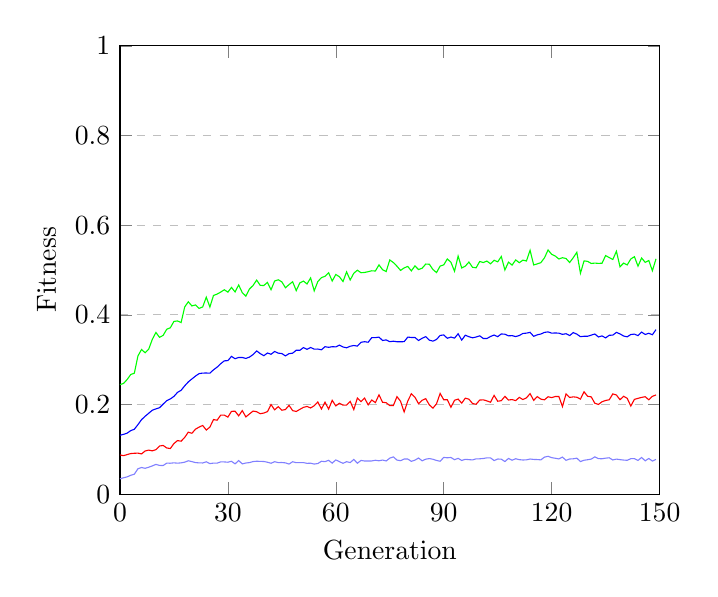
\begin{tikzpicture}
\begin{axis}[
	xlabel={Generation},
	ylabel={Fitness},
	xmin=0, xmax=150,
	ymin=0, ymax=1,
	xtick={0.0,30.0,60.0,90.0,120.0,150.0},
	ytick={0.0,0.2,0.4,0.6000000000000001,0.8,1.0},
	ymajorgrids=true,
	grid style=dashed,
]

\addplot[
	color=green,
	]
	coordinates {
	(0,0.2441430555555556)(1,0.24682777777777773)(2,0.2556844444444445)(3,0.2668408333333333)(4,0.26971194444444446)(5,0.3082621296296296)(6,0.3225826851851852)(7,0.31531055555555554)(8,0.3234491666666667)(9,0.34532611111111117)(10,0.36060129629629634)(11,0.34978851851851867)(12,0.3540337962962963)(13,0.3677262962962963)(14,0.3710710185185184)(15,0.38529361111111105)(16,0.3862841666666667)(17,0.38283925925925927)(18,0.41752462962962966)(19,0.428976111111111)(20,0.419823611111111)(21,0.421965)(22,0.4143839814814814)(23,0.4174908333333332)(24,0.4393206481481482)(25,0.4172834259259259)(26,0.44312101851851865)(27,0.44617611111111116)(28,0.4506470370370371)(29,0.455871388888889)(30,0.45049601851851845)(31,0.4611457407407406)(32,0.4510065740740741)(33,0.46656907407407405)(34,0.4495473148148148)(35,0.44169018518518527)(36,0.4574708333333333)(37,0.46540203703703703)(38,0.4773607407407407)(39,0.46555148148148146)(40,0.4654059259259259)(41,0.4722998148148148)(42,0.4559755555555555)(43,0.4753555555555556)(44,0.47817462962962964)(45,0.473502037037037)(46,0.4603316666666666)(47,0.46740694444444447)(48,0.47373814814814813)(49,0.45393231481481483)(50,0.471237962962963)(51,0.47523509259259245)(52,0.46876037037037027)(53,0.4822818518518518)(54,0.45335907407407405)(55,0.4741485185185186)(56,0.48286453703703697)(57,0.48590611111111115)(58,0.49384083333333334)(59,0.47535546296296305)(60,0.48990787037037037)(61,0.48489407407407414)(62,0.4741303703703705)(63,0.49583759259259264)(64,0.4776655555555556)(65,0.49271027777777787)(66,0.49949787037037047)(67,0.49384138888888895)(68,0.49445592592592597)(69,0.49617870370370365)(70,0.49817138888888884)(71,0.49766046296296296)(72,0.5113411111111111)(73,0.500651574074074)(74,0.4965871296296296)(75,0.5223609259259259)(76,0.5165574999999999)(77,0.5084306481481481)(78,0.49899462962962954)(79,0.5046119444444445)(80,0.5079146296296296)(81,0.4980151851851852)(82,0.5090812037037037)(83,0.5009174999999999)(84,0.503929351851852)(85,0.5132300925925927)(86,0.5127416666666667)(87,0.5010292592592592)(88,0.49425518518518524)(89,0.5086314814814815)(90,0.511398888888889)(91,0.524597037037037)(92,0.5172125925925926)(93,0.4972375000000001)(94,0.53113)(95,0.5044247222222222)(96,0.5085783333333334)(97,0.517645925925926)(98,0.5060715740740741)(99,0.5048063888888888)(100,0.5189533333333334)(101,0.5166016666666667)(102,0.5198737962962963)(103,0.5137926851851853)(104,0.5216055555555557)(105,0.5181823148148148)(106,0.5300853703703704)(107,0.5000392592592592)(108,0.517411574074074)(109,0.5108712037037038)(110,0.5224427777777777)(111,0.5162531481481482)(112,0.5219337037037036)(113,0.5200362037037036)(114,0.5439453703703704)(115,0.5112422222222222)(116,0.5135154629629629)(117,0.5163411111111111)(118,0.5269914814814816)(119,0.5446783333333334)(120,0.5349224074074074)(121,0.5311508333333333)(122,0.5245001851851853)(123,0.5273876851851852)(124,0.5254970370370372)(125,0.5165710185185185)(126,0.5274259259259261)(127,0.5393774074074075)(128,0.4926662962962964)(129,0.5202709259259259)(130,0.5191621296296296)(131,0.5145357407407408)(132,0.51537)(133,0.5146901851851851)(134,0.5150850000000001)(135,0.5321728703703704)(136,0.5276329629629629)(137,0.5234199074074074)(138,0.5417262037037037)(139,0.5070412962962964)(140,0.515358611111111)(141,0.5112061111111111)(142,0.5245323148148148)(143,0.5296587962962963)(144,0.50847)(145,0.5266644444444445)(146,0.5169488888888889)(147,0.5211596296296296)(148,0.49827888888888894)(149,0.5247004629629629)
	};
\addplot[
	color=blue,
	]
	coordinates {
	(0,0.13127846836419754)(1,0.1333747222222222)(2,0.13608741512345676)(3,0.14161955246913582)(4,0.14477288966049381)(5,0.1549582986111111)(6,0.16614708333333333)(7,0.17363413194444444)(8,0.18044368441358022)(9,0.18717145061728396)(10,0.19019156250000002)(11,0.1927088927469136)(12,0.2007640162037037)(13,0.20846334104938274)(14,0.21231795138888887)(15,0.21793449459876543)(16,0.22693515432098763)(17,0.23160451774691357)(18,0.2415812538580247)(19,0.25033516203703704)(20,0.256929537037037)(21,0.2633461766975309)(22,0.26881819830246917)(23,0.27001010416666665)(24,0.2701377160493827)(25,0.2698841473765432)(26,0.2772451003086419)(27,0.2831779591049382)(28,0.2908057214506173)(29,0.29732459104938275)(30,0.2977862422839507)(31,0.30727340663580244)(32,0.30207204089506173)(33,0.30474680555555556)(34,0.304740837191358)(35,0.30273066743827165)(36,0.3056308179012346)(37,0.31132324845679016)(38,0.3194544714506173)(39,0.31339081018518516)(40,0.30880822916666667)(41,0.31473314043209877)(42,0.31197343750000006)(43,0.31816760030864205)(44,0.314485574845679)(45,0.3135336111111111)(46,0.3083695717592593)(47,0.31332795524691354)(48,0.31438388117283955)(49,0.3209832908950617)(50,0.3207781250000001)(51,0.3268402816358025)(52,0.3230580285493827)(53,0.3271507021604938)(54,0.3233232831790124)(55,0.3236285455246914)(56,0.3220001195987654)(57,0.3288203780864198)(58,0.3274999035493827)(59,0.3288696527777778)(60,0.3284621836419754)(61,0.3324014236111112)(62,0.3281960223765432)(63,0.32638072530864193)(64,0.3299133140432099)(65,0.331514899691358)(66,0.33022265046296295)(67,0.338652488425926)(68,0.3399830671296296)(69,0.33881986111111106)(70,0.34908076388888887)(71,0.3490523842592593)(72,0.350279637345679)(73,0.34270211419753077)(74,0.3440252199074074)(75,0.3400651890432099)(76,0.3410836033950618)(77,0.3399348225308643)(78,0.3398956828703704)(79,0.3400863155864197)(80,0.35027839120370363)(81,0.34946490740740743)(82,0.34939836805555563)(83,0.34274479552469134)(84,0.3476821797839506)(85,0.3512834606481482)(86,0.3434785841049383)(87,0.34124378086419754)(88,0.3450586265432099)(89,0.35398214891975305)(90,0.3550880979938271)(91,0.34767659336419754)(92,0.3503979050925926)(93,0.348011087962963)(94,0.35771145447530867)(95,0.3435729822530864)(96,0.35448888503086423)(97,0.3511472106481481)(98,0.34871958333333336)(99,0.3504243402777777)(100,0.3530512577160494)(101,0.34719766203703706)(102,0.34712371527777774)(103,0.35165174768518515)(104,0.35484258101851845)(105,0.3512418016975308)(106,0.3572960108024691)(107,0.3566915972222222)(108,0.3530711728395062)(109,0.3535107831790123)(110,0.35149434799382717)(111,0.3537671489197531)(112,0.35841792052469135)(113,0.359072712191358)(114,0.36087368441358014)(115,0.35199880787037036)(116,0.3553720601851852)(117,0.3571418981481482)(118,0.36077617283950614)(119,0.36191393904320984)(120,0.3590803665123457)(121,0.3594515470679012)(122,0.3590792669753086)(123,0.3563858757716049)(124,0.3577250694444444)(125,0.3536795408950617)(126,0.3603565740740741)(127,0.35689125)(128,0.3512367168209876)(129,0.35216902391975313)(130,0.3521456018518519)(131,0.3546637808641976)(132,0.357209375)(133,0.35054763117283955)(134,0.3529041936728396)(135,0.3485195949074075)(136,0.354331361882716)(137,0.354703074845679)(138,0.3607946720679012)(139,0.3574038811728395)(140,0.3526259259259259)(141,0.3508932137345679)(142,0.35606215277777775)(143,0.3569487037037038)(144,0.3535136265432099)(145,0.3613897415123457)(146,0.35616597222222224)(147,0.35880001157407404)(148,0.35556418595679007)(149,0.366934837962963)
	};
\addplot[
	color=red,
	]
	coordinates {
	(0,0.08747935185185185)(1,0.08578907407407409)(2,0.08821074074074071)(3,0.09046972222222216)(4,0.09113379629629632)(5,0.09147620370370373)(6,0.08970175925925924)(7,0.09625555555555555)(8,0.09821000000000002)(9,0.09649907407407407)(10,0.09917148148148144)(11,0.10732962962962962)(12,0.10860935185185182)(13,0.10304814814814815)(14,0.10162379629629632)(15,0.11279898148148149)(16,0.11946990740740739)(17,0.11808453703703704)(18,0.12658685185185187)(19,0.13820509259259253)(20,0.135730925925926)(21,0.1449135185185185)(22,0.14950694444444437)(23,0.15319120370370376)(24,0.1430002777777778)(25,0.1495432407407407)(26,0.1663436111111111)(27,0.16489444444444445)(28,0.17608222222222225)(29,0.17627351851851852)(30,0.17182861111111114)(31,0.18462472222222223)(32,0.185029537037037)(33,0.1746507407407408)(34,0.18639277777777777)(35,0.17223675925925927)(36,0.17884425925925923)(37,0.1852830555555556)(38,0.1838048148148148)(39,0.17938231481481484)(40,0.18089185185185191)(41,0.18407157407407407)(42,0.19966851851851847)(43,0.18805388888888888)(44,0.1951181481481482)(45,0.1871653703703704)(46,0.18870435185185183)(47,0.19806231481481482)(48,0.18628768518518513)(49,0.18437481481481477)(50,0.18907212962962963)(51,0.19351296296296297)(52,0.19561740740740746)(53,0.19217296296296305)(54,0.19722351851851852)(55,0.20559648148148155)(56,0.18984398148148152)(57,0.20504148148148146)(58,0.18962916666666663)(59,0.20921824074074072)(60,0.19670222222222217)(61,0.20273601851851858)(62,0.19849259259259264)(63,0.1987068518518518)(64,0.20684398148148148)(65,0.18855685185185178)(66,0.21436222222222223)(67,0.20659916666666667)(68,0.21413712962962966)(69,0.199110462962963)(70,0.20995268518518523)(71,0.2041217592592593)(72,0.22145814814814815)(73,0.2049467592592592)(74,0.20389398148148152)(75,0.1975588888888889)(76,0.19763277777777777)(77,0.2173712962962963)(78,0.20722324074074078)(79,0.18325416666666666)(80,0.20768814814814815)(81,0.22387370370370382)(82,0.21614796296296301)(83,0.20165314814814814)(84,0.20935703703703704)(85,0.2129622222222222)(86,0.19903759259259263)(87,0.1918175925925926)(88,0.20153361111111107)(89,0.22456500000000001)(90,0.21047361111111101)(91,0.21050046296296293)(92,0.19372324074074082)(93,0.20925898148148145)(94,0.2120040740740741)(95,0.202965462962963)(96,0.21403749999999996)(97,0.2118236111111111)(98,0.20205037037037032)(99,0.20051259259259252)(100,0.20983546296296302)(101,0.21033462962962962)(102,0.20801861111111108)(103,0.204965)(104,0.22027222222222226)(105,0.20724212962962973)(106,0.20844453703703708)(107,0.21798416666666665)(108,0.2098821296296296)(109,0.21094222222222228)(110,0.2085760185185185)(111,0.21584000000000006)(112,0.21099148148148145)(113,0.21485879629629626)(114,0.22412972222222227)(115,0.2092285185185185)(116,0.21751379629629625)(117,0.21185722222222225)(118,0.2104523148148148)(119,0.21718601851851846)(120,0.21525731481481486)(121,0.217705)(122,0.21776759259259254)(123,0.1953724074074074)(124,0.22369092592592596)(125,0.21566166666666658)(126,0.21696999999999994)(127,0.21612)(128,0.2119396296296296)(129,0.22822962962962962)(130,0.21824611111111122)(131,0.21695018518518513)(132,0.20272018518518517)(133,0.20000666666666675)(134,0.20603833333333332)(135,0.20892129629629633)(136,0.21046305555555558)(137,0.2236623148148148)(138,0.2209992592592593)(139,0.2106548148148148)(140,0.2182756481481482)(141,0.2136969444444445)(142,0.19644138888888887)(143,0.2113913888888889)(144,0.21362416666666664)(145,0.21579740740740747)(146,0.2172712037037037)(147,0.2104859259259259)(148,0.21816287037037035)(149,0.22118490740740743)
	};
\addplot[
	color=blue!50,
	]
	coordinates {
	(0,0.03413586961051367)(1,0.0365671984073854)(2,0.03849898573960934)(3,0.04197659249769223)(4,0.044500014957003724)(5,0.056633410519081495)(6,0.05937590061442925)(7,0.05759558079046282)(8,0.06007141406316464)(9,0.0629514965616286)(10,0.06640546734188198)(11,0.0640354013611381)(12,0.06383769225877471)(13,0.06909600710452217)(14,0.068978050442231)(15,0.06978293476952112)(16,0.0690750422687728)(17,0.06974505855121801)(18,0.07132492434238859)(19,0.07440309457268642)(20,0.07253752255743234)(21,0.07036672541234817)(22,0.06970259225052895)(23,0.06953821035717854)(24,0.07219341967366243)(25,0.06807538691685347)(26,0.06924577575019156)(27,0.06910949246620296)(28,0.07188053884317172)(29,0.07182121376794272)(30,0.07120400027034733)(31,0.07323250475577352)(32,0.06750885707182232)(33,0.07495000722725546)(34,0.06744023135171469)(35,0.06941074637611783)(36,0.07031945780649067)(37,0.0726216570528628)(38,0.07338145614828899)(39,0.07304114184100113)(40,0.07281639990709848)(41,0.07116315605617554)(42,0.06891735220031213)(43,0.07230585384883134)(44,0.07036690961659178)(45,0.07048884377995819)(46,0.06974618216088835)(47,0.06710954333799245)(48,0.07221920616289212)(49,0.07015303650103498)(50,0.07035238607614512)(51,0.07032899122419742)(52,0.06867883775195147)(53,0.06906602875997155)(54,0.06705812819933639)(55,0.06826992659338442)(56,0.07326818397644906)(57,0.07251806635807968)(58,0.0754525166735892)(59,0.06919497278158097)(60,0.07633736469539824)(61,0.07247212467193542)(62,0.06872839459498188)(63,0.07240427524560283)(64,0.07044187356893224)(65,0.07734839940848882)(66,0.06893582896722762)(67,0.07516925506220869)(68,0.07383017296732089)(69,0.0739026900709543)(70,0.07403409196726676)(71,0.07556172266151953)(72,0.07440767971258704)(73,0.07601312945585773)(74,0.07397588789400658)(75,0.08024353229360587)(76,0.08306867957793532)(77,0.07599539860553499)(78,0.07460338277826942)(79,0.07824875939503924)(80,0.07833568479011829)(81,0.07305219457170964)(82,0.07581642467070994)(83,0.08057993508789517)(84,0.07427589316756789)(85,0.07803694330966027)(86,0.07928837803359637)(87,0.07784022971899908)(88,0.07517542648496264)(89,0.07334490671003518)(90,0.08188702969010442)(91,0.08107755785404094)(92,0.08176945105351792)(93,0.07679278423279216)(94,0.07983049059427348)(95,0.07517438830712489)(96,0.0776371330631039)(97,0.07695284848234168)(98,0.07634643407179227)(99,0.07876950805090008)(100,0.07880618145520644)(101,0.07952800736319034)(102,0.0809309688497334)(103,0.08095951777195316)(104,0.07483260517096527)(105,0.07830445553723211)(106,0.07810592705862222)(107,0.07268475694763099)(108,0.07961316807287629)(109,0.07570613028822226)(110,0.07895540029086244)(111,0.07688796562528746)(112,0.07614277251337234)(113,0.07644379210981177)(114,0.07832911966043837)(115,0.0774014043738445)(116,0.07708581485451221)(117,0.07643814122360718)(118,0.08258452241993577)(119,0.08437330671117521)(120,0.0813798377374968)(121,0.08005506510286625)(122,0.07849926527987672)(123,0.08256465176904132)(124,0.07546010100271121)(125,0.07834941374540125)(126,0.07880511842526564)(127,0.08024552585957057)(128,0.07268467374464359)(129,0.07559637765809654)(130,0.07674477892458695)(131,0.0781729248441479)(132,0.0831174488330373)(133,0.07913322459272627)(134,0.07893106618391725)(135,0.08026240194779075)(136,0.0810834784642632)(137,0.07623485876452132)(138,0.07813889628514975)(139,0.07694681128680762)(140,0.07600424004175738)(141,0.07546922086369719)(142,0.07910120959612868)(143,0.07927043677779962)(144,0.075165331085765)(145,0.08176949606382307)(146,0.07427767353150186)(147,0.07955233814558915)(148,0.07373065206231608)(149,0.07745120735391954)
	};
\end{axis}
\end{tikzpicture}
}
		\caption{Some sample caption}
		\label{fig:hard-fitness}
	\end{subfigure}%
}
\caption{Figure shows results from a simulation in the hard environment (p.1)}
\end{figure}

\newpage
\vspace*{-2.0cm}
\textbf{\Huge Results - Hard environment (2)}
\vspace{1.5cm}
\begin{tikzpicture}[remember picture,overlay]
   \node[anchor=south east,inner sep=20pt] at (current page.south east)
              {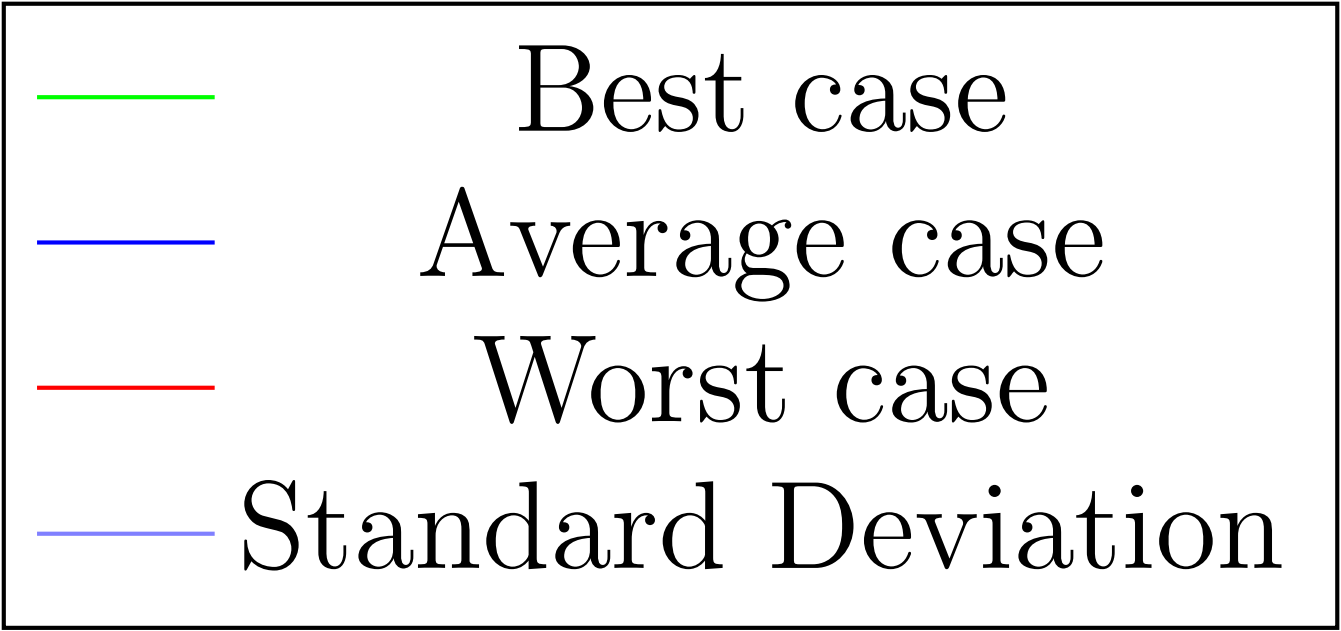
\includegraphics[scale=0.1]{chapters/res/generated_graph_legend.png}};
\end{tikzpicture}

\begin{figure}[H]
\vspace*{-1cm}
	\makebox[\linewidth][c]{%
	\begin{subfigure}[b]{0.7\textwidth}
		\centering
		\resizebox{0.9\linewidth}{!}{
        \begin{filecontents}{coord-hard-out.dat}
             x  y  r 
	 30 3 0.200000 
	 30 2 2.733333 
	 30 4 0.016667 
	 30 6 0.016667 
	 60 3 0.300000 
	 60 2 2.833333 
	 60 5 0.016667 
	 60 4 0.016667 
	 90 3 0.266667 
	 90 2 3.350000 
	 90 5 0.016667 
	 120 3 0.266667 
	 120 2 3.466667 
	 120 5 0.016667 
	 120 4 0.033333 
	 149 3 0.266667 
	 149 2 3.233333 
	 149 5 0.016667 
	 149 4 0.050000 

        \end{filecontents}
        
        \begin{tikzpicture}
        \begin{axis}[% scatter/use mapped color={draw=black,fill=mapped color},
        xmin=0, xmax=170,
        ymin=1, ymax=9,
        xlabel={Generation},
        ylabel={Group size},
        xtick={0.0,30.0,60.0,90.0,120.0,150.0},
        ytick={0.0,1.0,2.0,3.0,4.0,5.0, 6.0, 7.0, 8.0},]
        \addplot[scatter,scatter src=explicit, mark=*,only marks,
        % we use ’point meta’ as color data...
        point meta=\thisrow{r},
        % ... therefore, we can’t use it as argument for nodes near coords
        % ... which requires to define a visualization dependency:
        visualization depends on={value \thisrow{r} \as \r},
        scatter/@pre marker code/.append style=
        {/tikz/mark size=\r*3}
        ]
        table [x=x, y=y]
        {coord-hard-out.dat};
        \end{axis}
        \end{tikzpicture}	}
		\caption{Some sample caption}
		\label{fig:group-sizes-hard}
	\end{subfigure}%
	\begin{subfigure}[b]{0.7\textwidth}
		\centering
		\resizebox{0.9\linewidth}{!}{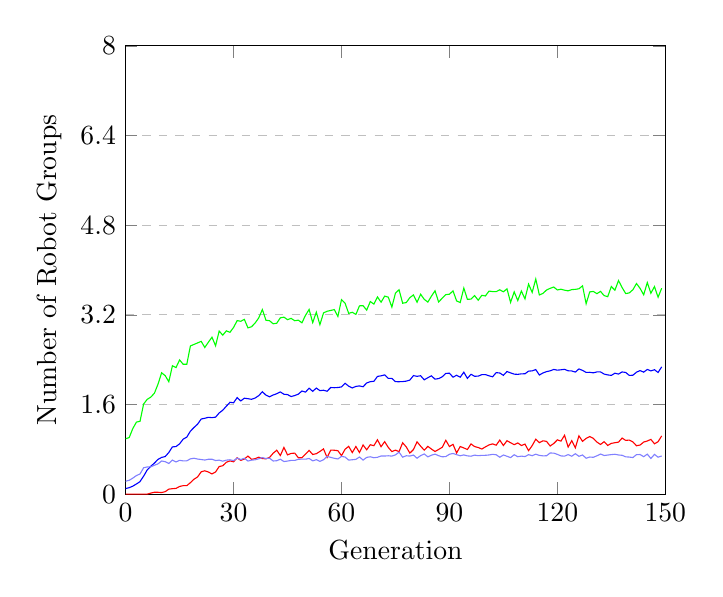
\begin{tikzpicture}
\begin{axis}[
	xlabel={Generation},
	ylabel={Number of Robot Groups},
	xmin=0, xmax=150,
	ymin=0, ymax=8,
	xtick={0.0,30.0,60.0,90.0,120.0,150.0},
	ytick={0.0,1.6,3.2,4.800000000000001,6.4,8.0},
	ymajorgrids=true,
	grid style=dashed,
]

\addplot[
	color=green,
	]
	coordinates {
	(0,0.9885)(1,1.0105)(2,1.1705)(3,1.2850833333333334)(4,1.3003333333333333)(5,1.6087499999999997)(6,1.6916666666666667)(7,1.73125)(8,1.8010000000000002)(9,1.96225)(10,2.1654166666666663)(11,2.1138333333333335)(12,2.0058333333333334)(13,2.290166666666667)(14,2.2583333333333333)(15,2.39425)(16,2.3168333333333333)(17,2.3175833333333338)(18,2.6443333333333334)(19,2.6715)(20,2.698166666666667)(21,2.7266666666666666)(22,2.616916666666667)(23,2.711)(24,2.8004999999999995)(25,2.647416666666666)(26,2.9100833333333336)(27,2.8361666666666667)(28,2.91375)(29,2.88775)(30,2.9744166666666665)(31,3.096333333333333)(32,3.0847500000000005)(33,3.1181666666666668)(34,2.9665)(35,2.987083333333333)(36,3.0541666666666663)(37,3.144833333333333)(38,3.293916666666667)(39,3.102416666666666)(40,3.094583333333333)(41,3.039833333333333)(42,3.0495)(43,3.1460000000000004)(44,3.1583333333333328)(45,3.1134999999999997)(46,3.13675)(47,3.0943333333333336)(48,3.1045833333333333)(49,3.0574166666666662)(50,3.1907499999999995)(51,3.2953333333333332)(52,3.060583333333334)(53,3.2466666666666666)(54,3.0235000000000003)(55,3.233416666666666)(56,3.2635000000000005)(57,3.27775)(58,3.2928333333333333)(59,3.170416666666666)(60,3.4700833333333327)(61,3.4057500000000003)(62,3.22525)(63,3.245166666666667)(64,3.2065833333333327)(65,3.360416666666667)(66,3.3628333333333327)(67,3.283583333333334)(68,3.4359166666666665)(69,3.3921666666666663)(70,3.5194166666666664)(71,3.4246666666666674)(72,3.5332500000000002)(73,3.5153333333333334)(74,3.3373333333333335)(75,3.5867500000000003)(76,3.647083333333333)(77,3.4069166666666666)(78,3.4181666666666666)(79,3.506250000000001)(80,3.5550000000000006)(81,3.42275)(82,3.566833333333333)(83,3.476333333333333)(84,3.427083333333333)(85,3.5321666666666665)(86,3.62825)(87,3.4285833333333327)(88,3.496833333333333)(89,3.559916666666667)(90,3.5672499999999996)(91,3.626749999999999)(92,3.4471666666666665)(93,3.418916666666667)(94,3.677583333333333)(95,3.4754166666666677)(96,3.48075)(97,3.5424166666666674)(98,3.4597500000000005)(99,3.5475000000000003)(100,3.536083333333333)(101,3.6227500000000004)(102,3.614583333333333)(103,3.613083333333334)(104,3.6454999999999993)(105,3.6109999999999993)(106,3.6636666666666673)(107,3.420416666666666)(108,3.6105)(109,3.4541666666666666)(110,3.6239999999999997)(111,3.48375)(112,3.747833333333334)(113,3.5999166666666667)(114,3.838333333333333)(115,3.554)(116,3.5820833333333333)(117,3.6424999999999996)(118,3.6724166666666664)(119,3.6955833333333343)(120,3.6435)(121,3.6565000000000007)(122,3.639166666666667)(123,3.6272500000000005)(124,3.649749999999999)(125,3.654166666666667)(126,3.6645833333333333)(127,3.7170833333333335)(128,3.397333333333333)(129,3.6089166666666666)(130,3.617083333333334)(131,3.5771666666666673)(132,3.6181666666666663)(133,3.54275)(134,3.5235)(135,3.704916666666667)(136,3.6390000000000002)(137,3.8111666666666664)(138,3.6860833333333334)(139,3.5785833333333334)(140,3.591083333333333)(141,3.6481666666666674)(142,3.7577500000000006)(143,3.671416666666667)(144,3.5568333333333335)(145,3.7747499999999996)(146,3.584916666666667)(147,3.7040833333333327)(148,3.5135)(149,3.674416666666666)
	};
\addplot[
	color=blue,
	]
	coordinates {
	(0,0.0986736111111111)(1,0.11563888888888892)(2,0.1426458333333333)(3,0.18130902777777777)(4,0.22395138888888888)(5,0.32067013888888884)(6,0.43254513888888896)(7,0.49868749999999995)(8,0.5538819444444445)(9,0.6199756944444443)(10,0.6553159722222224)(11,0.6706458333333334)(12,0.7433020833333333)(13,0.8430902777777779)(14,0.8488055555555555)(15,0.8977881944444445)(16,0.981670138888889)(17,1.0169166666666667)(18,1.1233020833333334)(19,1.18953125)(20,1.2479861111111112)(21,1.339875)(22,1.3537916666666665)(23,1.3705347222222222)(24,1.3649027777777778)(25,1.3736041666666663)(26,1.4487222222222222)(27,1.4972916666666665)(28,1.5694756944444443)(29,1.6386666666666667)(30,1.6303541666666668)(31,1.7230937499999999)(32,1.662611111111111)(33,1.712079861111111)(34,1.702982638888889)(35,1.6919722222222224)(36,1.7151874999999999)(37,1.7570520833333334)(38,1.827579861111111)(39,1.7665347222222223)(40,1.7368854166666665)(41,1.7686770833333334)(42,1.7917881944444443)(43,1.824125)(44,1.781965277777778)(45,1.776152777777778)(46,1.7410486111111105)(47,1.7593124999999998)(48,1.7837604166666667)(49,1.8403402777777778)(50,1.8206562499999999)(51,1.8905277777777778)(52,1.8341423611111114)(53,1.89275)(54,1.8469409722222223)(55,1.8537777777777777)(56,1.8366354166666665)(57,1.902451388888889)(58,1.8989236111111105)(59,1.9026631944444448)(60,1.9133194444444444)(61,1.9780381944444443)(62,1.9263368055555552)(63,1.8948888888888893)(64,1.9223298611111113)(65,1.931163194444444)(66,1.9163229166666667)(67,1.9829479166666664)(68,2.0066631944444446)(69,2.0135868055555557)(70,2.1003055555555554)(71,2.111045138888889)(72,2.12778125)(73,2.06596875)(74,2.0651805555555556)(75,2.0068402777777776)(76,2.0059027777777776)(77,2.008583333333333)(78,2.016284722222222)(79,2.034979166666667)(80,2.115166666666667)(81,2.1018298611111117)(82,2.1125659722222223)(83,2.0398645833333338)(84,2.0773993055555557)(85,2.1102499999999997)(86,2.0515000000000003)(87,2.0621666666666667)(88,2.0943125000000005)(89,2.1544409722222224)(90,2.157934027777778)(91,2.087427083333333)(92,2.1207604166666667)(93,2.0860347222222226)(94,2.175947916666667)(95,2.065892361111111)(96,2.1383576388888894)(97,2.1034548611111115)(98,2.1055868055555553)(99,2.1319270833333333)(100,2.1327881944444442)(101,2.1116354166666667)(102,2.093819444444444)(103,2.1682569444444444)(104,2.161482638888889)(105,2.119854166666667)(106,2.188097222222222)(107,2.1633472222222223)(108,2.1410104166666666)(109,2.137274305555555)(110,2.1465312500000002)(111,2.1476666666666664)(112,2.1951875)(113,2.199246527777778)(114,2.2231423611111114)(115,2.125541666666667)(116,2.1619826388888885)(117,2.186225694444444)(118,2.20009375)(119,2.224652777777777)(120,2.211857638888889)(121,2.2187812500000006)(122,2.227243055555556)(123,2.2010902777777774)(124,2.198652777777778)(125,2.1774444444444443)(126,2.2343993055555558)(127,2.208243055555556)(128,2.172427083333333)(129,2.1739618055555563)(130,2.164527777777778)(131,2.180510416666667)(132,2.180861111111111)(133,2.14246875)(134,2.127434027777778)(135,2.1188958333333328)(136,2.1578958333333333)(137,2.1426180555555554)(138,2.1806875)(139,2.1707534722222226)(140,2.118270833333333)(141,2.1218229166666664)(142,2.176100694444445)(143,2.204652777777778)(144,2.1769930555555557)(145,2.225496527777778)(146,2.1988090277777776)(147,2.219822916666667)(148,2.171017361111111)(149,2.2716458333333334)
	};
\addplot[
	color=red,
	]
	coordinates {
	(0,0.0)(1,0.0)(2,0.0)(3,0.0)(4,0.0)(5,0.0)(6,0.0)(7,0.018416666666666668)(8,0.033916666666666664)(9,0.032999999999999995)(10,0.027666666666666666)(11,0.043833333333333335)(12,0.08908333333333332)(13,0.09741666666666668)(14,0.10224999999999998)(15,0.13725)(16,0.1509166666666667)(17,0.1515)(18,0.20441666666666666)(19,0.2655833333333334)(20,0.30783333333333335)(21,0.3978333333333333)(22,0.41658333333333325)(23,0.39424999999999993)(24,0.36108333333333337)(25,0.3956666666666667)(26,0.4923333333333334)(27,0.5069999999999999)(28,0.5691666666666666)(29,0.59275)(30,0.5777500000000001)(31,0.6479999999999999)(32,0.6024166666666668)(33,0.6264166666666667)(34,0.6792499999999999)(35,0.6212500000000001)(36,0.63325)(37,0.6598333333333333)(38,0.6344166666666666)(39,0.6306666666666667)(40,0.6546666666666665)(41,0.7289999999999999)(42,0.7833333333333334)(43,0.6891666666666665)(44,0.8331666666666665)(45,0.7008333333333333)(46,0.7259166666666667)(47,0.7321666666666664)(48,0.6498333333333333)(49,0.6499999999999999)(50,0.7134166666666667)(51,0.7802499999999999)(52,0.7077500000000001)(53,0.7216666666666667)(54,0.7610833333333334)(55,0.8069166666666667)(56,0.6530833333333333)(57,0.7851666666666667)(58,0.78375)(59,0.7748333333333333)(60,0.6873333333333334)(61,0.8006666666666666)(62,0.8529166666666665)(63,0.7414166666666665)(64,0.8497500000000001)(65,0.7426666666666666)(66,0.8765833333333333)(67,0.7916666666666666)(68,0.8815000000000001)(69,0.8643333333333333)(70,0.9700833333333332)(71,0.8468333333333334)(72,0.936)(73,0.8344166666666667)(74,0.7593333333333332)(75,0.7856666666666666)(76,0.7581666666666667)(77,0.9169166666666665)(78,0.8422499999999999)(79,0.7321666666666667)(80,0.7949999999999999)(81,0.9334999999999999)(82,0.8554166666666665)(83,0.7841666666666668)(84,0.8524166666666667)(85,0.8040833333333332)(86,0.7609166666666667)(87,0.79725)(88,0.8359166666666668)(89,0.9601666666666667)(90,0.8495000000000001)(91,0.8886666666666665)(92,0.73475)(93,0.8495)(94,0.8240000000000001)(95,0.7965833333333333)(96,0.8959166666666666)(97,0.8487500000000001)(98,0.8320000000000001)(99,0.805)(100,0.8426666666666666)(101,0.8781666666666665)(102,0.8965)(103,0.8733333333333334)(104,0.9645833333333332)(105,0.8679166666666668)(106,0.95325)(107,0.9172500000000002)(108,0.8829166666666666)(109,0.9134166666666669)(110,0.8678333333333333)(111,0.893)(112,0.7754999999999999)(113,0.8655)(114,0.9804166666666667)(115,0.9194166666666667)(116,0.9515)(117,0.9411666666666667)(118,0.8586666666666664)(119,0.9035833333333334)(120,0.9685833333333335)(121,0.9459166666666666)(122,1.0505)(123,0.8401666666666664)(124,0.9539166666666667)(125,0.8270833333333335)(126,1.0401666666666665)(127,0.9424166666666667)(128,0.9944166666666667)(129,1.0269166666666667)(130,0.9955000000000003)(131,0.92825)(132,0.8865833333333333)(133,0.9358333333333333)(134,0.8685833333333333)(135,0.9058333333333333)(136,0.9175)(137,0.928)(138,1.0005000000000002)(139,0.9591666666666667)(140,0.96475)(141,0.9314166666666667)(142,0.86325)(143,0.8765833333333335)(144,0.9290833333333335)(145,0.94825)(146,0.9764166666666666)(147,0.8981666666666667)(148,0.9358333333333333)(149,1.0391666666666666)
	};
\addplot[
	color=blue!50,
	]
	coordinates {
	(0,0.23041392412848985)(1,0.24721100159067225)(2,0.2861116761865935)(3,0.33164751255320146)(4,0.35984079506965055)(5,0.47051954045550026)(6,0.48488246016221576)(7,0.4874163742115373)(8,0.5154807632045703)(9,0.5398266421295853)(10,0.5918608330814454)(11,0.5783346915141413)(12,0.5479438376439714)(13,0.6073861166960819)(14,0.5741424856902813)(15,0.6033033428402926)(16,0.5931742900711261)(17,0.5943975971711536)(18,0.6292707240264681)(19,0.6403525836181031)(20,0.6260904859028299)(21,0.6174786069081931)(22,0.6083391412007119)(23,0.6219109827361557)(24,0.6229182278230316)(25,0.5995172909632441)(26,0.6066471904322772)(27,0.5880839814735296)(28,0.6066834459681001)(29,0.6131782486278229)(30,0.5967339142181725)(31,0.6428149411469115)(32,0.6174482882016558)(33,0.6400339063152171)(34,0.590460488403954)(35,0.6066567662491295)(36,0.6125454424059454)(37,0.6312638691779325)(38,0.6527375174076562)(39,0.6342519803000547)(40,0.6418778732329667)(41,0.5914012979506952)(42,0.5960015133713243)(43,0.6229595259047211)(44,0.5820820589167834)(45,0.5898941906213113)(46,0.6025599915048048)(47,0.6013819339261692)(48,0.6213977235467489)(49,0.6250810102468466)(50,0.6237067206372977)(51,0.6361606977640398)(52,0.593971346662099)(53,0.6153793353132855)(54,0.5846692963689726)(55,0.6133141068974148)(56,0.6728735527322817)(57,0.6561553825320928)(58,0.639538948876635)(59,0.6279023022662097)(60,0.6738323266572568)(61,0.6619758918211559)(62,0.6066754960183073)(63,0.6137154296849585)(64,0.6198868780022028)(65,0.6625433921325612)(66,0.6078675409693064)(67,0.6556475599824937)(68,0.6664221930777681)(69,0.6495526218766009)(70,0.6575297105019131)(71,0.6808904316344891)(72,0.679895413083442)(73,0.6844791216127859)(74,0.6782801587635531)(75,0.7008178367928691)(76,0.7486661415936056)(77,0.6595091042539707)(78,0.6848958293334734)(79,0.6790717454154572)(80,0.6973805516508398)(81,0.6408704930154457)(82,0.6872716670624742)(83,0.7162641111393582)(84,0.6655913579410292)(85,0.6942284078621174)(86,0.7141166893482851)(87,0.6856483626428292)(88,0.6661895465349275)(89,0.670486950765176)(90,0.71151958224271)(91,0.7257803856184589)(92,0.7040319332261691)(93,0.6848891919768718)(94,0.6994385892151413)(95,0.6827655202921703)(96,0.6765905183100039)(97,0.69586918448832)(98,0.6863646601841195)(99,0.6916605642941964)(100,0.6929700213346228)(101,0.6988739938366116)(102,0.7102863999535943)(103,0.7025362865904404)(104,0.6584424950377278)(105,0.6981523492325586)(106,0.6759158192094806)(107,0.651872195030143)(108,0.7030164037357817)(109,0.6676260445977136)(110,0.6781853964289033)(111,0.6697806248232375)(112,0.7044167525074774)(113,0.6858992597822058)(114,0.7130620057939888)(115,0.6916777102388724)(116,0.6829768681278207)(117,0.6847285354850419)(118,0.7346048502560758)(119,0.7313658568233201)(120,0.7095214786845512)(121,0.682143647161689)(122,0.6775017455606567)(123,0.7054483502991999)(124,0.6764708831026437)(125,0.721443831703775)(126,0.6748070209769378)(127,0.6990119409674921)(128,0.641083930710199)(129,0.6622701986303058)(130,0.6569423081009023)(131,0.6842094593395093)(132,0.7155105131827088)(133,0.6894644232543202)(134,0.6976403082438506)(135,0.7053499096133211)(136,0.7112001819594219)(137,0.698843783266371)(138,0.6930339746099535)(139,0.6655341308666695)(140,0.6613080738053698)(141,0.653187858671551)(142,0.705187471338016)(143,0.7065478859016558)(144,0.6683018784227313)(145,0.7137387794154163)(146,0.6361007049684605)(147,0.7095809973737295)(148,0.6589089893419686)(149,0.6800941585709698)
	};
\end{axis}
\end{tikzpicture}
}
		\caption{Some sample caption}
		\label{fig:number-of-groups-hard}
	\end{subfigure}%
}
\\
\\
\\
\\
	\makebox[\linewidth][c]{%
	\begin{subfigure}[b]{0.7\textwidth}
		\centering
		\resizebox{0.9\linewidth}{!}{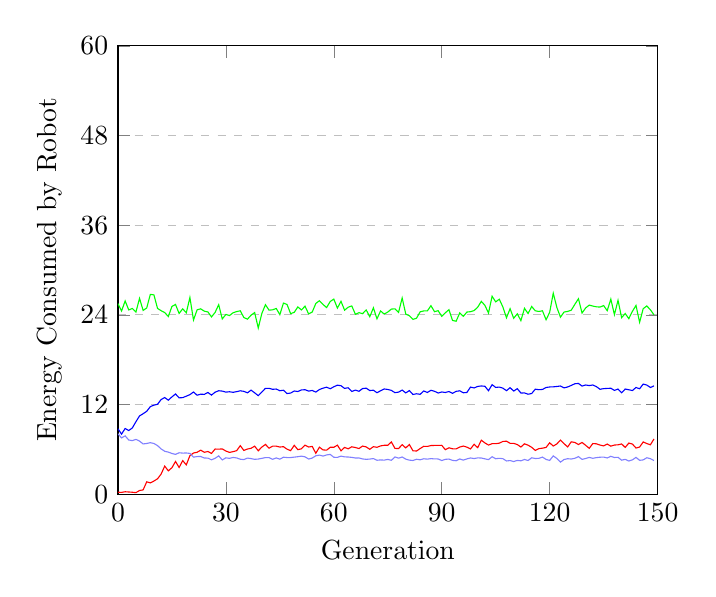
\begin{tikzpicture}
\begin{axis}[
	xlabel={Generation},
	ylabel={Energy Consumed by Robot},
	xmin=0, xmax=150,
	ymin=0, ymax=60,
	xtick={0.0,30.0,60.0,90.0,120.0,150.0},
	ytick={0.0,12.0,24.0,36.0,48.0,60.0},
	ymajorgrids=true,
	grid style=dashed,
]

\addplot[
	color=green,
	]
	coordinates {
	(0,25.5)(1,24.5)(2,25.850000000000005)(3,24.650000000000002)(4,24.849999999999998)(5,24.366666666666667)(6,26.199999999999996)(7,24.583333333333332)(8,24.916666666666664)(9,26.733333333333334)(10,26.666666666666664)(11,24.85)(12,24.55)(13,24.300000000000004)(14,23.766666666666666)(15,25.11666666666667)(16,25.38333333333333)(17,24.18333333333333)(18,24.800000000000004)(19,24.26666666666667)(20,26.316666666666663)(21,23.299999999999997)(22,24.666666666666664)(23,24.800000000000004)(24,24.48333333333333)(25,24.383333333333336)(26,23.716666666666672)(27,24.316666666666663)(28,25.350000000000005)(29,23.45)(30,24.05)(31,23.900000000000002)(32,24.26666666666667)(33,24.433333333333334)(34,24.533333333333328)(35,23.63333333333333)(36,23.416666666666668)(37,23.95)(38,24.3)(39,22.233333333333334)(40,24.18333333333333)(41,25.35)(42,24.616666666666664)(43,24.666666666666664)(44,24.849999999999998)(45,24.016666666666666)(46,25.566666666666663)(47,25.383333333333333)(48,24.150000000000002)(49,24.333333333333336)(50,25.05)(51,24.65)(52,25.150000000000002)(53,24.11666666666667)(54,24.36666666666667)(55,25.516666666666666)(56,25.88333333333333)(57,25.383333333333336)(58,24.96666666666667)(59,25.78333333333334)(60,26.100000000000005)(61,24.9)(62,25.799999999999997)(63,24.616666666666667)(64,25.016666666666666)(65,25.183333333333337)(66,24.066666666666666)(67,24.28333333333333)(68,24.15)(69,24.65)(70,23.733333333333334)(71,24.93333333333333)(72,23.46666666666667)(73,24.516666666666666)(74,24.099999999999998)(75,24.366666666666664)(76,24.766666666666662)(77,24.8)(78,24.333333333333336)(79,26.25)(80,24.099999999999998)(81,23.866666666666667)(82,23.383333333333336)(83,23.549999999999997)(84,24.4)(85,24.516666666666666)(86,24.516666666666666)(87,25.216666666666665)(88,24.41666666666666)(89,24.55)(90,23.799999999999997)(91,24.26666666666667)(92,24.683333333333334)(93,23.25)(94,23.133333333333333)(95,24.249999999999993)(96,23.8)(97,24.366666666666667)(98,24.416666666666668)(99,24.566666666666663)(100,25.016666666666662)(101,25.8)(102,25.266666666666666)(103,24.233333333333334)(104,26.483333333333338)(105,25.733333333333338)(106,26.08333333333333)(107,25.050000000000004)(108,23.599999999999998)(109,24.816666666666666)(110,23.533333333333328)(111,24.133333333333336)(112,23.21666666666667)(113,24.86666666666666)(114,24.166666666666668)(115,25.116666666666667)(116,24.533333333333335)(117,24.45)(118,24.533333333333335)(119,23.333333333333336)(120,24.333333333333336)(121,26.9)(122,24.983333333333338)(123,23.683333333333326)(124,24.366666666666667)(125,24.450000000000003)(126,24.616666666666667)(127,25.399999999999995)(128,26.150000000000002)(129,24.233333333333334)(130,24.916666666666668)(131,25.299999999999997)(132,25.166666666666664)(133,25.066666666666666)(134,25.033333333333335)(135,25.233333333333338)(136,24.55)(137,26.1)(138,24.016666666666666)(139,25.950000000000003)(140,23.616666666666664)(141,24.166666666666664)(142,23.48333333333333)(143,24.466666666666665)(144,25.25)(145,22.999999999999996)(146,24.81666666666667)(147,25.183333333333337)(148,24.666666666666668)(149,24.0)
	};
\addplot[
	color=blue,
	]
	coordinates {
	(0,8.743055555555554)(1,8.029861111111112)(2,8.782638888888886)(3,8.507638888888888)(4,8.861805555555556)(5,9.692361111111111)(6,10.463888888888892)(7,10.760416666666668)(8,11.084027777777779)(9,11.710416666666667)(10,11.904861111111108)(11,12.022916666666665)(12,12.661111111111113)(13,12.924305555555556)(14,12.574305555555558)(15,13.011805555555554)(16,13.402083333333332)(17,12.884027777777778)(18,12.914583333333336)(19,13.108333333333336)(20,13.313888888888886)(21,13.66527777777778)(22,13.237499999999999)(23,13.376388888888888)(24,13.349305555555556)(25,13.60138888888889)(26,13.254861111111113)(27,13.64236111111111)(28,13.835416666666669)(29,13.7875)(30,13.652083333333334)(31,13.7)(32,13.624305555555555)(33,13.71597222222222)(34,13.827777777777778)(35,13.752777777777775)(36,13.554861111111112)(37,13.918055555555554)(38,13.559027777777777)(39,13.173611111111112)(40,13.669444444444446)(41,14.160416666666668)(42,14.156944444444445)(43,14.027777777777777)(44,14.063888888888888)(45,13.835416666666665)(46,13.904166666666669)(47,13.462500000000002)(48,13.524305555555555)(49,13.800000000000002)(50,13.731250000000001)(51,13.941666666666666)(52,13.972916666666666)(53,13.78611111111111)(54,13.872222222222222)(55,13.658333333333335)(56,13.99722222222222)(57,14.179861111111112)(58,14.310416666666667)(59,14.104166666666668)(60,14.363888888888887)(61,14.58333333333333)(62,14.50763888888889)(63,14.15069444444444)(64,14.236111111111112)(65,13.739583333333332)(66,13.920833333333334)(67,13.766666666666662)(68,14.127083333333333)(69,14.179166666666667)(70,13.862499999999999)(71,13.90763888888889)(72,13.569444444444445)(73,13.82777777777778)(74,14.074999999999996)(75,14.00625)(76,13.880555555555555)(77,13.575694444444444)(78,13.652083333333332)(79,13.923611111111109)(80,13.54652777777778)(81,13.85486111111111)(82,13.33472222222222)(83,13.431944444444445)(84,13.357638888888893)(85,13.806249999999999)(86,13.605555555555554)(87,13.893749999999999)(88,13.762500000000003)(89,13.529166666666667)(90,13.671527777777776)(91,13.602777777777774)(92,13.72777777777778)(93,13.488888888888889)(94,13.752083333333335)(95,13.82916666666667)(96,13.565277777777776)(97,13.60486111111111)(98,14.32430555555556)(99,14.209722222222219)(100,14.41388888888889)(101,14.475694444444448)(102,14.431249999999999)(103,13.836805555555554)(104,14.65)(105,14.278472222222222)(106,14.327083333333334)(107,14.179166666666664)(108,13.845833333333333)(109,14.245138888888887)(110,13.794444444444444)(111,14.109722222222222)(112,13.531944444444443)(113,13.544444444444444)(114,13.37013888888889)(115,13.463194444444444)(116,14.043750000000001)(117,13.974305555555555)(118,14.011805555555554)(119,14.26597222222222)(120,14.341666666666667)(121,14.357638888888891)(122,14.408333333333333)(123,14.471527777777775)(124,14.218750000000002)(125,14.340972222222222)(126,14.54583333333333)(127,14.771527777777777)(128,14.813888888888888)(129,14.461805555555555)(130,14.606250000000001)(131,14.527083333333332)(132,14.604166666666666)(133,14.381250000000001)(134,14.031944444444447)(135,14.118749999999999)(136,14.146527777777777)(137,14.170833333333333)(138,13.880555555555555)(139,14.061805555555557)(140,13.556944444444444)(141,14.063194444444445)(142,13.96736111111111)(143,13.863888888888889)(144,14.271527777777777)(145,14.098611111111115)(146,14.727083333333336)(147,14.595138888888888)(148,14.266666666666667)(149,14.490277777777777)
	};
\addplot[
	color=red,
	]
	coordinates {
	(0,0.24999999999999997)(1,0.2333333333333333)(2,0.31666666666666665)(3,0.2833333333333333)(4,0.24999999999999997)(5,0.2)(6,0.4833333333333333)(7,0.5666666666666667)(8,1.6500000000000001)(9,1.5)(10,1.75)(11,2.05)(12,2.683333333333333)(13,3.7499999999999996)(14,3.1166666666666667)(15,3.533333333333333)(16,4.366666666666666)(17,3.5666666666666655)(18,4.483333333333332)(19,3.9166666666666656)(20,5.15)(21,5.5)(22,5.599999999999998)(23,5.883333333333334)(24,5.6000000000000005)(25,5.7)(26,5.449999999999999)(27,6.033333333333333)(28,6.016666666666666)(29,6.050000000000002)(30,5.766666666666667)(31,5.583333333333333)(32,5.6833333333333345)(33,5.8166666666666655)(34,6.4833333333333325)(35,5.8500000000000005)(36,6.033333333333334)(37,6.133333333333334)(38,6.416666666666666)(39,5.8)(40,6.299999999999999)(41,6.6499999999999995)(42,6.149999999999999)(43,6.416666666666666)(44,6.416666666666667)(45,6.299999999999998)(46,6.3500000000000005)(47,6.016666666666667)(48,5.8166666666666655)(49,6.533333333333333)(50,5.949999999999999)(51,6.066666666666666)(52,6.55)(53,6.300000000000001)(54,6.383333333333335)(55,5.466666666666667)(56,6.283333333333333)(57,5.916666666666666)(58,5.883333333333332)(59,6.266666666666666)(60,6.266666666666666)(61,6.55)(62,5.800000000000001)(63,6.25)(64,6.066666666666666)(65,6.333333333333334)(66,6.233333333333332)(67,6.1)(68,6.433333333333333)(69,6.316666666666666)(70,5.999999999999999)(71,6.349999999999998)(72,6.266666666666666)(73,6.449999999999999)(74,6.533333333333333)(75,6.533333333333332)(76,6.9833333333333325)(77,6.116666666666666)(78,6.1)(79,6.616666666666665)(80,6.183333333333333)(81,6.633333333333334)(82,5.8)(83,5.766666666666667)(84,6.1)(85,6.3999999999999995)(86,6.383333333333333)(87,6.499999999999999)(88,6.516666666666667)(89,6.5166666666666675)(90,6.533333333333332)(91,5.95)(92,6.2)(93,6.0666666666666655)(94,6.05)(95,6.3)(96,6.433333333333334)(97,6.283333333333332)(98,6.05)(99,6.666666666666665)(100,6.216666666666666)(101,7.216666666666666)(102,6.8500000000000005)(103,6.5666666666666655)(104,6.749999999999999)(105,6.75)(106,6.816666666666667)(107,7.050000000000001)(108,7.083333333333333)(109,6.800000000000001)(110,6.8)(111,6.633333333333334)(112,6.3)(113,6.733333333333332)(114,6.549999999999999)(115,6.266666666666667)(116,5.85)(117,6.083333333333334)(118,6.15)(119,6.249999999999999)(120,6.866666666666666)(121,6.433333333333334)(122,6.716666666666667)(123,7.233333333333333)(124,6.750000000000001)(125,6.3166666666666655)(126,7.0)(127,6.916666666666667)(128,6.633333333333333)(129,6.916666666666667)(130,6.533333333333332)(131,6.133333333333333)(132,6.766666666666668)(133,6.733333333333333)(134,6.566666666666668)(135,6.45)(136,6.699999999999998)(137,6.416666666666668)(138,6.566666666666667)(139,6.600000000000001)(140,6.716666666666665)(141,6.249999999999998)(142,6.833333333333333)(143,6.699999999999999)(144,6.166666666666666)(145,6.299999999999999)(146,6.983333333333333)(147,6.766666666666667)(148,6.6000000000000005)(149,7.383333333333334)
	};
\addplot[
	color=blue!50,
	]
	coordinates {
	(0,8.082774971063547)(1,7.5202066241319425)(2,7.79438782086935)(3,7.2410752085784456)(4,7.158201443596098)(5,7.329572864357157)(6,7.094120120173457)(7,6.716227492640775)(8,6.777598765221324)(9,6.883963701471235)(10,6.7740578899198685)(11,6.493609949648281)(12,6.048786329796665)(13,5.732358313706953)(14,5.6240454688748835)(15,5.439607138477879)(16,5.318545661760092)(17,5.532668690735819)(18,5.490484814806867)(19,5.504579505465947)(20,5.4505354703853826)(21,4.945450163433636)(22,5.025373844131298)(23,5.037933502931269)(24,4.830677606955687)(25,4.823215266556611)(26,4.584162253456718)(27,4.794934163357561)(28,5.118633270944958)(29,4.574574343687546)(30,4.858546965154467)(31,4.784109112477449)(32,4.906274752023848)(33,4.84097940419843)(34,4.671518328223549)(35,4.617489340909896)(36,4.823983962487431)(37,4.753867019889358)(38,4.653416126207805)(39,4.693673634979387)(40,4.7888107293775635)(41,4.888470123380413)(42,4.887135081159738)(43,4.656197409901727)(44,4.846605647296779)(45,4.675779416223535)(46,4.937243358975931)(47,4.893568261029841)(48,4.8915015339371894)(49,4.950987854753406)(50,5.0078440134134405)(51,5.08444066190008)(52,4.988326068594998)(53,4.695197738144902)(54,4.8272792437473)(55,5.132052312327927)(56,5.2213030339061275)(57,5.091486504677867)(58,5.244218034664606)(59,5.31438867012139)(60,4.9311016089949335)(61,4.916061261908784)(62,5.0878201314657705)(63,4.983317380900556)(64,4.966564717307446)(65,4.916350823841731)(66,4.832757476663486)(67,4.842915881461363)(68,4.706624338552414)(69,4.655845104711397)(70,4.691315381134466)(71,4.755769224131112)(72,4.533447143520904)(73,4.576712943093048)(74,4.547302341566114)(75,4.649196016443172)(76,4.525629360957749)(77,4.971015326366647)(78,4.811685981250474)(79,4.973242820181177)(80,4.683121611426587)(81,4.547618466022444)(82,4.49838411562389)(83,4.665782950449021)(84,4.591395098490995)(85,4.731787303606224)(86,4.681697902494333)(87,4.749275703211938)(88,4.712240909854335)(89,4.705696063403978)(90,4.495112771400719)(91,4.654699971380674)(92,4.694444240337387)(93,4.514399585594827)(94,4.4647307912404965)(95,4.709138330859537)(96,4.546279932165309)(97,4.717304242742753)(98,4.841678069760113)(99,4.758222432275121)(100,4.847945146398865)(101,4.831660543892366)(102,4.719283384041859)(103,4.616121147414768)(104,5.003767556649848)(105,4.735590157804179)(106,4.792470378701926)(107,4.742197779322269)(108,4.435849003612433)(109,4.491856577480856)(110,4.356940723536874)(111,4.510412588515327)(112,4.456255090167716)(113,4.635596570211798)(114,4.499045877858894)(115,4.859471393251463)(116,4.767886428299354)(117,4.784940581443324)(118,4.955752696626624)(119,4.6440829535373185)(120,4.510056723348685)(121,5.111893744400532)(122,4.772726487213811)(123,4.279219353870288)(124,4.6325691153498925)(125,4.738321999401243)(126,4.69606778576483)(127,4.794289376579589)(128,5.017787096900144)(129,4.649009445095565)(130,4.766579768836438)(131,4.914488897468409)(132,4.796091824807534)(133,4.884362528124775)(134,4.938756285798858)(135,4.956155966457181)(136,4.837243297961255)(137,5.062544808145106)(138,4.900953729295759)(139,4.925797609383625)(140,4.540595755872046)(141,4.650631363593984)(142,4.427806158293592)(143,4.5848686920624555)(144,4.9144975398960336)(145,4.526865748465059)(146,4.576604940246586)(147,4.86935360575204)(148,4.741177213702874)(149,4.497284498151326)
	};
\end{axis}
\end{tikzpicture}
}
		\caption{Some sample caption}
	\end{subfigure}%
	\begin{subfigure}[b]{0.7\textwidth}
		\centering
		\resizebox{0.9\linewidth}{!}{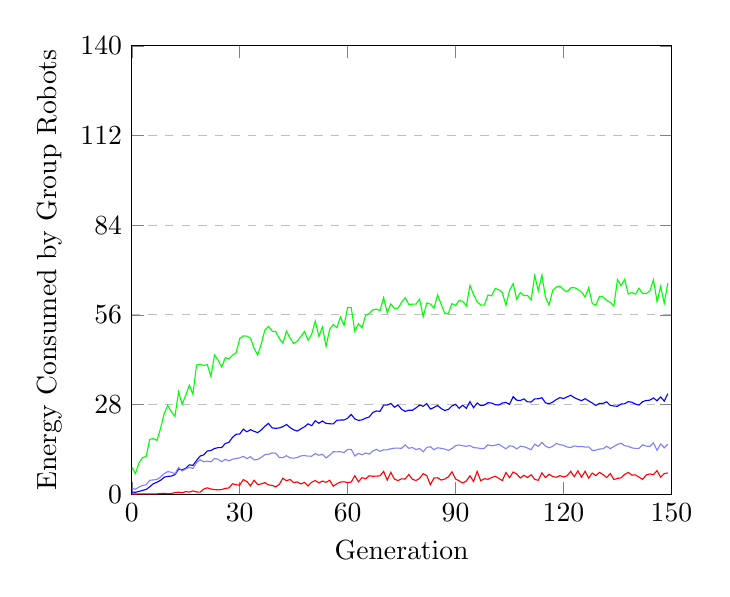
\begin{tikzpicture}
\begin{axis}[
	xlabel={Generation},
	ylabel={Energy Consumed by Group Robots},
	xmin=0, xmax=150,
	ymin=0, ymax=140,
	xtick={0.0,30.0,60.0,90.0,120.0,150.0},
	ytick={0.0,28.0,56.0,84.0,112.0,140.0},
	ymajorgrids=true,
	grid style=dashed,
]

\addplot[
	color=green,
	]
	coordinates {
	(0,8.416666666666668)(1,6.416666666666666)(2,9.75)(3,11.416666666666666)(4,11.783333333333333)(5,17.116666666666664)(6,17.35)(7,16.766666666666666)(8,20.533333333333335)(9,25.1)(10,27.71666666666667)(11,25.683333333333337)(12,24.283333333333335)(13,31.916666666666657)(14,28.033333333333335)(15,30.86666666666666)(16,34.016666666666666)(17,31.166666666666668)(18,40.30000000000001)(19,40.53333333333333)(20,40.18333333333334)(21,40.43333333333334)(22,36.74999999999999)(23,43.449999999999996)(24,41.81666666666667)(25,39.68333333333334)(26,42.64999999999999)(27,42.233333333333334)(28,43.36666666666667)(29,44.15)(30,48.6)(31,49.41666666666667)(32,49.33333333333333)(33,48.699999999999996)(34,45.51666666666667)(35,43.433333333333344)(36,46.95)(37,51.266666666666666)(38,52.35)(39,50.9)(40,50.74999999999999)(41,48.633333333333326)(42,47.14999999999999)(43,50.849999999999994)(44,48.71666666666667)(45,47.033333333333324)(46,47.733333333333334)(47,49.233333333333334)(48,50.800000000000004)(49,48.06666666666666)(50,49.916666666666664)(51,54.05)(52,49.300000000000004)(53,52.166666666666664)(54,46.10000000000001)(55,51.50000000000001)(56,52.95)(57,51.95000000000001)(58,55.31666666666667)(59,52.68333333333334)(60,58.3)(61,58.21666666666666)(62,50.83333333333334)(63,53.23333333333334)(64,51.95000000000001)(65,55.849999999999994)(66,56.43333333333334)(67,57.583333333333336)(68,57.76666666666667)(69,57.29999999999999)(70,61.35)(71,56.61666666666665)(72,59.4)(73,58.01666666666667)(74,58.06666666666666)(75,59.89999999999999)(76,61.333333333333336)(77,59.21666666666667)(78,59.31666666666666)(79,59.33333333333333)(80,60.900000000000006)(81,55.38333333333334)(82,59.7)(83,59.35000000000001)(84,58.100000000000016)(85,62.199999999999996)(86,59.300000000000004)(87,56.43333333333334)(88,56.46666666666667)(89,59.49999999999999)(90,58.900000000000006)(91,60.499999999999986)(92,60.166666666666686)(93,58.81666666666666)(94,65.18333333333334)(95,62.366666666666674)(96,60.03333333333334)(97,59.05)(98,59.033333333333324)(99,62.19999999999999)(100,61.91666666666668)(101,64.21666666666667)(102,63.85)(103,62.916666666666664)(104,58.98333333333332)(105,63.56666666666667)(106,65.73333333333333)(107,60.866666666666674)(108,62.91666666666666)(109,62.01666666666665)(110,62.04999999999999)(111,60.58333333333333)(112,68.25000000000001)(113,63.51666666666666)(114,68.39999999999999)(115,61.41666666666667)(116,59.066666666666656)(117,63.63333333333333)(118,64.68333333333334)(119,64.98333333333333)(120,63.85)(121,63.20000000000002)(122,64.41666666666667)(123,64.48333333333332)(124,63.93333333333333)(125,63.116666666666646)(126,61.56666666666667)(127,64.45)(128,59.516666666666666)(129,58.96666666666666)(130,61.76666666666667)(131,61.583333333333336)(132,60.51666666666667)(133,59.88333333333334)(134,58.68333333333332)(135,67.00000000000001)(136,65.05)(137,67.08333333333333)(138,62.48333333333333)(139,62.949999999999996)(140,62.449999999999996)(141,64.29999999999998)(142,62.68333333333333)(143,62.666666666666664)(144,63.43333333333334)(145,66.95)(146,60.099999999999994)(147,64.85000000000001)(148,59.63333333333333)(149,65.86666666666667)
	};
\addplot[
	color=blue,
	]
	coordinates {
	(0,0.658333333333333)(1,0.5701388888888889)(2,0.8465277777777777)(3,1.1604166666666667)(4,1.4659722222222222)(5,2.298611111111111)(6,3.2395833333333335)(7,3.703472222222222)(8,4.323611111111111)(9,5.261805555555556)(10,5.556249999999999)(11,5.622222222222221)(12,6.095833333333333)(13,7.788194444444445)(14,7.589583333333332)(15,8.059027777777777)(16,9.150694444444447)(17,8.980555555555554)(18,10.518055555555556)(19,11.87986111111111)(20,12.250000000000002)(21,13.489583333333334)(22,13.600694444444446)(23,14.252777777777778)(24,14.516666666666664)(25,14.557638888888889)(26,15.816666666666665)(27,16.17916666666667)(28,17.72222222222222)(29,18.692361111111104)(30,18.78125)(31,20.277777777777775)(32,19.45763888888889)(33,20.112499999999994)(34,19.611805555555556)(35,19.200000000000003)(36,20.04305555555555)(37,21.18819444444445)(38,22.086805555555554)(39,20.68125)(40,20.542361111111113)(41,20.670833333333338)(42,21.06180555555556)(43,21.749305555555555)(44,20.79930555555556)(45,20.075)(46,19.695138888888888)(47,20.37777777777778)(48,21.011805555555554)(49,21.934027777777782)(50,21.36597222222222)(51,22.92152777777778)(52,22.132638888888888)(53,22.834722222222222)(54,22.088194444444444)(55,21.977777777777778)(56,21.918750000000003)(57,23.041666666666668)(58,23.149305555555557)(59,23.15833333333334)(60,23.719444444444445)(61,24.87847222222222)(62,23.498611111111106)(63,23.025694444444444)(64,23.181250000000006)(65,23.727777777777785)(66,24.104166666666668)(67,25.486111111111114)(68,25.957638888888887)(69,25.856249999999996)(70,27.774305555555554)(71,27.802083333333332)(72,28.329861111111107)(73,27.13541666666666)(74,27.824305555555554)(75,26.496527777777786)(76,25.834722222222215)(77,26.19444444444445)(78,26.182638888888892)(79,26.923611111111118)(80,27.806250000000002)(81,27.43402777777778)(82,28.27986111111111)(83,26.56041666666667)(84,27.05138888888889)(85,27.7)(86,26.73472222222222)(87,26.102777777777778)(88,26.45902777777778)(89,27.524999999999995)(90,28.063194444444445)(91,26.778472222222216)(92,27.75902777777778)(93,26.788888888888888)(94,28.895138888888887)(95,26.987499999999997)(96,28.467361111111117)(97,27.629166666666666)(98,27.814583333333335)(99,28.55972222222222)(100,28.447222222222223)(101,27.950694444444448)(102,27.816666666666666)(103,28.460416666666667)(104,28.629166666666666)(105,28.008333333333333)(106,30.4375)(107,29.33472222222222)(108,29.244444444444447)(109,29.736111111111114)(110,28.792361111111113)(111,28.782638888888886)(112,29.731944444444448)(113,29.786111111111115)(114,30.112499999999997)(115,28.506944444444446)(116,28.23611111111111)(117,28.74236111111111)(118,29.5375)(119,30.147222222222222)(120,29.835416666666667)(121,30.367361111111116)(122,30.875)(123,30.13958333333333)(124,29.6125)(125,29.17569444444445)(126,29.812499999999993)(127,29.097222222222225)(128,28.45138888888889)(129,27.695138888888888)(130,28.321527777777774)(131,28.338888888888885)(132,28.833333333333336)(133,27.717361111111106)(134,27.513194444444444)(135,27.429861111111116)(136,28.125694444444445)(137,28.208333333333332)(138,28.893055555555552)(139,28.7)(140,28.120833333333334)(141,27.793055555555558)(142,28.895833333333332)(143,29.23055555555556)(144,29.351388888888888)(145,30.03125)(146,29.150694444444444)(147,30.340972222222227)(148,29.04652777777778)(149,31.355555555555554)
	};
\addplot[
	color=red,
	]
	coordinates {
	(0,0.05)(1,0.03333333333333333)(2,0.08333333333333334)(3,0.06666666666666667)(4,0.06666666666666667)(5,0.08333333333333333)(6,0.08333333333333333)(7,0.08333333333333333)(8,0.23333333333333334)(9,0.26666666666666666)(10,0.13333333333333333)(11,0.21666666666666667)(12,0.4666666666666666)(13,0.6166666666666667)(14,0.39999999999999997)(15,0.7833333333333334)(16,0.6333333333333334)(17,1.0166666666666668)(18,0.6666666666666667)(19,0.6166666666666668)(20,1.5833333333333333)(21,1.966666666666667)(22,1.6000000000000003)(23,1.4166666666666672)(24,1.3333333333333335)(25,1.4333333333333336)(26,1.8)(27,1.9333333333333338)(28,3.2333333333333334)(29,2.933333333333333)(30,2.8000000000000003)(31,4.533333333333332)(32,3.933333333333333)(33,2.566666666666667)(34,4.333333333333334)(35,2.95)(36,3.2)(37,3.6)(38,2.8833333333333333)(39,2.7500000000000004)(40,2.2500000000000004)(41,3.033333333333333)(42,4.966666666666667)(43,4.166666666666666)(44,4.599999999999999)(45,3.5999999999999988)(46,3.7999999999999994)(47,3.1833333333333336)(48,3.6500000000000004)(49,2.55)(50,3.733333333333334)(51,4.249999999999999)(52,3.483333333333333)(53,4.083333333333333)(54,3.683333333333333)(55,4.333333333333333)(56,2.4833333333333334)(57,3.2333333333333325)(58,3.766666666666666)(59,3.8666666666666667)(60,3.616666666666667)(61,3.766666666666667)(62,5.766666666666668)(63,3.8500000000000005)(64,5.133333333333333)(65,4.783333333333333)(66,5.7333333333333325)(67,5.5666666666666655)(68,5.633333333333334)(69,5.699999999999999)(70,7.1000000000000005)(71,4.383333333333333)(72,6.800000000000001)(73,4.700000000000001)(74,4.233333333333333)(75,4.783333333333333)(76,4.7)(77,6.133333333333333)(78,4.65)(79,4.249999999999999)(80,4.916666666666667)(81,6.416666666666666)(82,5.75)(83,2.933333333333333)(84,5.033333333333333)(85,5.1)(86,4.3999999999999995)(87,4.7)(88,5.416666666666666)(89,7.0)(90,4.733333333333333)(91,4.133333333333334)(92,3.4499999999999997)(93,4.133333333333332)(94,5.733333333333334)(95,3.9666666666666672)(96,7.1000000000000005)(97,4.166666666666667)(98,4.833333333333333)(99,4.633333333333333)(100,5.15)(101,5.6)(102,4.933333333333334)(103,4.216666666666667)(104,6.766666666666666)(105,5.15)(106,6.899999999999999)(107,6.3)(108,5.050000000000001)(109,5.883333333333333)(110,5.183333333333334)(111,6.033333333333333)(112,4.599999999999999)(113,4.316666666666667)(114,6.6499999999999995)(115,5.15)(116,6.233333333333333)(117,5.483333333333333)(118,5.266666666666666)(119,5.7666666666666675)(120,5.366666666666667)(121,5.716666666666668)(122,7.116666666666668)(123,5.45)(124,7.250000000000003)(125,5.3)(126,7.116666666666665)(127,5.033333333333333)(128,6.550000000000001)(129,5.783333333333333)(130,6.783333333333332)(131,6.099999999999999)(132,5.166666666666666)(133,6.433333333333334)(134,4.5666666666666655)(135,4.8999999999999995)(136,5.1000000000000005)(137,6.166666666666668)(138,6.7666666666666675)(139,5.966666666666666)(140,6.0)(141,5.299999999999999)(142,4.6)(143,5.983333333333333)(144,6.316666666666668)(145,6.083333333333333)(146,7.333333333333333)(147,5.283333333333334)(148,6.366666666666667)(149,6.649999999999999)
	};
\addplot[
	color=blue!50,
	]
	coordinates {
	(0,1.8601966159801082)(1,1.5163419762637518)(2,2.2091691350828957)(3,2.6958063862333015)(4,2.9458106808425866)(5,4.313683621636453)(6,4.435500862272461)(7,4.576654200488078)(8,5.3180033444474395)(9,6.3900950828301815)(10,7.02890192907096)(11,6.837116420505935)(12,6.328077746661747)(13,8.32386719582467)(14,7.237258902877992)(15,7.886208299343419)(16,8.326140958610646)(17,8.044868246661826)(18,9.797627326607714)(19,10.758907920252442)(20,10.105380593374594)(21,10.312721449052768)(22,10.078927656519749)(23,11.140162518301844)(24,10.88786185204116)(25,10.14357257340158)(26,10.875713581577317)(27,10.37765529232587)(28,10.919238599765098)(29,11.087983143034062)(30,11.345875688973543)(31,11.780169635160215)(32,11.102078353116031)(33,11.686401133263859)(34,10.678557946360826)(35,10.81046878523493)(36,11.491594863556033)(37,12.309061128971573)(38,12.441947625661825)(39,12.860151932204921)(40,12.760134926172922)(41,11.464140765398104)(42,11.38390350420378)(43,12.006591969941647)(44,11.313358716160915)(45,11.222193398664597)(46,11.442489025055119)(47,11.934520389398447)(48,12.039195718508752)(49,11.856021879635257)(50,11.841063943828438)(51,12.655403943749969)(52,12.140918969878689)(53,12.43978895481577)(54,11.29102104694152)(55,12.154282510866292)(56,13.231063714449649)(57,13.207712442464995)(58,13.258765641237952)(59,12.998781428697)(60,13.970061906186034)(61,13.992940597122933)(62,11.911103478032341)(63,12.706502609177186)(64,12.305319293118504)(65,12.834345318169243)(66,12.467594801931792)(67,13.456519962541998)(68,13.994796949476587)(69,13.358780942314294)(70,13.844842042305082)(71,13.82941831104123)(72,14.177046029863332)(73,14.34289520285072)(74,14.366245348115307)(75,14.304527394934956)(76,15.348276499721534)(77,14.318823140345089)(78,14.547902156003465)(79,13.89281802526852)(80,14.267076108522438)(81,13.214902427306571)(82,14.561178681038655)(83,14.814678691033198)(84,13.854375567324796)(85,14.485973366134768)(86,14.284938117987002)(87,14.068640171396936)(88,13.661118328978594)(89,14.258134498429184)(90,15.135941516588245)(91,15.360108104292625)(92,15.104933161146343)(93,14.924949149840202)(94,15.174171589269758)(95,14.51621757621291)(96,14.43381817866796)(97,14.245286577325139)(98,14.303784615613148)(99,15.401022208804767)(100,15.09451707702169)(101,15.23432730382014)(102,15.602576172263074)(103,14.877397023809547)(104,14.156965281439962)(105,15.100554540970895)(106,14.935822800916256)(107,14.111838294116474)(108,14.953866405723002)(109,14.804507222204647)(110,14.39525968711036)(111,13.854764165107364)(112,15.631027849569106)(113,14.915081304915837)(114,16.16642590877393)(115,14.987237939013728)(116,14.473695206499638)(117,14.954992021884873)(118,15.824753868290697)(119,15.441740669748999)(120,15.238550711195515)(121,14.71474101442031)(122,14.541467856591378)(123,15.068460113747818)(124,14.844117530974119)(125,14.879509790326424)(126,14.683831633661464)(127,14.759560090293876)(128,13.623946683694937)(129,13.725045955867545)(130,14.088076418789141)(131,14.145253649613768)(132,14.943135522379686)(133,14.205493755440234)(134,14.866369110776336)(135,15.510663901398535)(136,15.923158357337043)(137,15.106624437453897)(138,14.963573238938908)(139,14.446569280989072)(140,14.2870744170796)(141,14.289379393980964)(142,15.391643107599894)(143,14.992839917008427)(144,14.901915170439073)(145,16.004978482580785)(146,13.672355675946182)(147,15.655688251721253)(148,14.466025884741802)(149,15.606029739275346)
	};
\end{axis}
\end{tikzpicture}
}
		\caption{Some sample caption}
	\end{subfigure}%
}
\caption{Figure shows results from a simulation in the hard environment (p.2)}
\end{figure}
